\ifdefined\ishandout
\documentclass[11pt,handout]{beamer}
\else
\documentclass[11pt]{beamer}
\fi

% 日本語対応
\usepackage{luatexja}
\usepackage{luatexja-fontspec}
\renewcommand{\kanjifamilydefault}{\gtdefault}

\usepackage{mathptmx}
\renewcommand{\sfdefault}{lmss}
\renewcommand{\familydefault}{\sfdefault}
\usepackage[T1]{fontenc}
\usepackage{amsmath}
\usepackage{amssymb}
\usepackage{graphicx}
\usepackage{xcolor,multirow,colortbl}
\PassOptionsToPackage{normalem}{ulem}
\usepackage{ulem}
\usepackage{caption}
\captionsetup{labelformat=empty}
\usepackage{bbm}
\usepackage{upgreek}
\setbeamertemplate{section in toc}[sections numbered]
\makeatletter
\usepackage{caption} 
\usepackage{bm}
\usepackage{subfig}
\captionsetup[table]{skip=10pt}
\newcommand\makebeamertitle{\frame{\maketitle}}%
\AtBeginDocument{%
	\let\origtableofcontents=\tableofcontents
	\def\tableofcontents{\@ifnextchar[{\origtableofcontents}{\gobbletableofcontents}}
	\def\gobbletableofcontents#1{\origtableofcontents}
}

\def\Tiny{\fontsize{7pt}{8pt}\selectfont}
\def\Normal{\fontsize{8pt}{10pt}\selectfont}

\usetheme{Madrid}
\usecolortheme{lily}
\useinnertheme{rounded}

\setbeamertemplate{footline}{\hfill\Normal{\insertframenumber/\inserttotalframenumber}}
\setbeamertemplate{navigation symbols}{}

\newenvironment{changemargin}[2]{%
	\begin{list}{}{%
			\setlength{\topsep}{0pt}%
			\setlength{\leftmargin}{#1}%
			\setlength{\rightmargin}{#2}%
			\setlength{\listparindent}{\parindent}%
			\setlength{\itemindent}{\parindent}%
			\setlength{\parsep}{\parskip}% 
		}%
		\item[]}{\end{list}}

\setbeamertemplate{footline}{\hfill\insertframenumber/\inserttotalframenumber}
\setbeamertemplate{navigation symbols}{}

\usepackage{graphicx}
\usepackage{epsfig}
\usepackage{bm}
\usepackage{epsf}
\usepackage{float}
\usepackage[final]{pdfpages}
\usepackage{multirow}
\usepackage{colortbl}
\usepackage{xkeyval}
\usepackage{listings}
\usepackage{ifthen}
\usepackage{tikz}

\usepackage{setspace}
\usepackage{ragged2e}

\setbeamersize{text margin left=1em,text margin right=1em} 

% Table formatting
\usepackage{booktabs}

% Decimal align
\usepackage{dcolumn}
\newcolumntype{d}[0]{D{.}{.}{5}}

\global\long\def\expec#1{\mathbb{E}\left[#1\right]}
\global\long\def\var#1{\mathrm{Var}\left[#1\right]}
\global\long\def\cov#1{\mathrm{Cov}\left[#1\right]}
\global\long\def\prob#1{\mathrm{Prob}\left[#1\right]}
\global\long\def\one{\mathbf{1}}
\global\long\def\diag{\operatorname{diag}}
\global\long\def\expe#1#2{\mathbb{E}_{#1}\left[#2\right]}
\DeclareMathOperator*{\plim}{\text{plim}}

\usepackage{appendixnumberbeamer}
\renewcommand{\thefootnote}{}

\setbeamertemplate{footline}
{
	\leavevmode%
\hfill
	\insertframenumber{}\hspace*{2ex}\vspace{1ex}
}

\definecolor{blue}{RGB}{0, 0, 210}
\definecolor{red}{RGB}{170, 0, 0}

\makeatother

\usepackage[english]{babel}

\usepackage{tikz}
\newcommand*\circled[1]{\tikz[baseline=(char.base)]{             \node[circle,ball color=structure.fg, shade,   color=white,inner sep=1.2pt] (char) {\tiny #1};}} 

\makeatletter
\let\save@measuring@true\measuring@true
\def\measuring@true{%
	\save@measuring@true
	\def\beamer@sortzero##1{\beamer@ifnextcharospec{\beamer@sortzeroread{##1}}{}}%
	\def\beamer@sortzeroread##1<##2>{}%
	\def\beamer@finalnospec{}%
}
\makeatother

\definecolor{amethyst}{rgb}{0.6, 0.4, 0.8}

\setbeamersize{text margin left= .8em,text margin right=1em} 
\newenvironment{wideitemize}{\itemize\addtolength{\itemsep}{10pt}}{\enditemize}
\newenvironment{wideitemizeshort}{\itemize}{\enditemize}

\newcommand{\indep}{\perp\!\!\!\!\perp} 

\DeclareMathOperator*{\argmax}{arg\,max}
\DeclareMathOperator*{\argmin}{arg\,min}

\begin{document}
	
	%% タイトルスライド
	\begin{frame}[noframenumbering]{}
		\vspace{0.5cm}
		\title[]{第5章：多変量回帰}
		\author{Jonathan Roth}
		\date{数理計量経済学 I \\ ブラウン大学\\} 
		\titlepage {\small{}\ }\thispagestyle{empty} \vspace{-30pt}
		
	\end{frame}
	
	
	\begin{frame}{アウトライン}

	1. 多変量回帰と OLS の導出
	\vspace{0.8cm}
	
	2. 回帰と因果関係
	\vspace{0.8cm}
	
	3. 回帰に関するその他のトピック
	
	\end{frame}
		
	\begin{frame}{1つの「説明変数」を超えて}
		\begin{wideitemize}
			
			\item
			これまでは、1つのスカラー $X_i$ に対して、条件付き期待値関数（CEF） $E[Y_i|X_i =x ] \approx \alpha + x \beta$ を近似する方法として回帰を扱ってきました。
			\begin{itemize}
					\item 
					そして、推定対象 ($\alpha, \beta$) を OLS で推定する方法を示しました。
				\end{itemize}
			
			\pause
			\item
			次に、これを一般化して、ベクトル $\mathbf{X}_i = (1, X_{i1}, \dots, X_{iK})'$ に対して $E[Y_i | \mathbf{X}_i = \mathbf{x}] \approx \mathbf{x}' \bm{\beta}$ を近似・推定する方法を見ていきます。
				\begin{itemize}\smallskip
					\item 
					注意：いつものように、ベクトルや行列は\textbf{太字}で表記します。
				\end{itemize}
			
			\pause
			\item
			これには主に2つの動機があります： \medskip
			\end{wideitemize}	

			\pause
\begin{enumerate}
			\item
			回帰を用いて因果的効果を識別したいが、条件付き非交絡性は複数のコントロール変数を入れなければ妥当ではない場合。 \smallskip
			\begin{itemize}
				\item 
				ブラウン大対URIの例では、高校のGPA、世帯所得、SATスコア、人種などをコントロールしたいかもしれません。
			\end{itemize}
			\medskip
			
			\pause
			\item
			\textbf{非線形}な CEF の近似が欲しい場合：例 $E[Y_i\mid X_i]\approx\alpha+X_i\beta+X_i^2\gamma$ \smallskip
			\begin{itemize}
			\item $\mathbf{X}_i = (1, X_{i}, X_{i}^2)'$ と設定することで、回帰を「騙して」これを行わせることができます。
			\end{itemize}
			\end{enumerate}
			
		
		
	\end{frame}
	
		
	\begin{frame}{年齢別・対数賃金}
		\centering
		\includegraphics[width = 0.8 \linewidth]{logwages}
		
	\end{frame}
	
	\begin{frame}{OLS 回帰（線形フィット）}
		\centering
		\includegraphics[width = 0.8 \linewidth]{logwages-linear}
		
	\end{frame}
	
		\begin{frame}{OLS 回帰（2次式フィット）}
		\centering
		\includegraphics[width = 0.8 \linewidth]{logwages-quadratic}
		
	\end{frame}

\begin{frame}{最小二乗問題としての多変量回帰}
	\begin{wideitemize}
		\item
		単変量 OLS では、以下を解きました：
		$$(\alpha, \beta) = \argmin_{a,b} E[ (Y_i - (a + b X_i))^2 ] $$
		
		CEF が線形であれば $E[Y|X] = \alpha + \beta X$ となり、そうでなければ $\alpha + \beta X$ が最良の線形近似を与えることを見ました。
		
		\pause
		\item
		ここで多変量の場合を考えます：
		\begin{align*}
		\boldsymbol\beta= \arg \min_{\mathbf{b}} E\left[(Y_i-\mathbf{X}_i^\prime\boldsymbol b)^2\right]
		\end{align*}
	
		\item
		単変量の場合と同様の手順で、CEF が $\mathbf{X}$ に関して線形であれば $E[Y| \mathbf{X}] = \mathbf{X}'\boldsymbol{\beta}$ となり、そうでなければ $\mathbf{X}'\boldsymbol{\beta}$ が CEF を平均二乗誤差（MSE）の意味で最小化する近似となることを示せます。
	 
	\end{wideitemize}
\end{frame}
	
	\begin{frame}{回帰係数の算出}
		\begin{wideitemize}
			\item
			\emph{母集団回帰係数} $\boldsymbol\beta$ は以下の最小二乗問題を解くことで得られます：
						
			$$\bm{\beta} = \argmin_{\mathbf{b}} E[ (Y_i - \mathbf{X}_i '\mathbf{b})^2]$$
			
			\pause
			\item
			$\bm{\beta}$ について微分（勾配）をとり、0 と置きます：
			\begin{align*}
				& \dfrac{d}{d \bm{\beta}} E[ (Y_i - \mathbf{X}_i '\bm{\beta})^2] = \mathbf{0} \pause{} \\
				\Rightarrow & E[ \dfrac{d}{d \bm{\beta}} (Y_i - \mathbf{X}_i '\bm{\beta})^2] = \mathbf{0} \pause{} \\
				\Rightarrow & E[-2 \mathbf{X}_i (Y_i - \mathbf{X}_i '\bm{\beta})] = \mathbf{0} \pause{}\\
				\Rightarrow & E[\mathbf{X}_i Y_i] = E[\mathbf{X}_i \mathbf{X}_i ']\bm{\beta}
			\end{align*}
		
	
		\end{wideitemize}
	\end{frame}
	
	
	\begin{frame}{母集団と標本における多変量回帰}
		\begin{wideitemize}
			\item
			$\bm{\beta}$ について解くと、母平均を用いた式が得られます：
			$$\bm{\beta} = E[ \bm{X}_i \bm{X}_i'  ]^{-1} E[\bm{X}_i Y_i] $$
			\vspace{-0.3cm}
			\begin{itemize}
			\item 少し計算すれば、$\mathbf{X}_i=(1,X_i)^\prime$ のときに単変量の公式 $\beta=\frac{Cov(X_i,Y_i)}{Var(X_i)}$ および $\alpha=E[Y_i]-E[X_i]\beta$ に一致することを示せます。
			\end{itemize}
			\pause\smallskip
			\item
			$\bm{\beta}$ を推定するために、母平均を標本平均に置き換えます：
			
			\pause
			$$ \bm{\hat\beta} = \left( \frac{1}{N} \sum_{i=1}^N \bm{X}_i \bm{X}_i' \right)^{-1}  \left( \frac{1}{N} \sum_{i=1}^N \bm{X}_i Y_i \right)$$
			
			\pause\smallskip
			\item 
			これで、任意のベクトル $\mathbf{X}_i=(1,X_{i1},\dots,X_{iK})^\prime$ に対して $E[Y_i\mid \mathbf{X}_i]\approx \mathbf{X}_i^\prime\boldsymbol{\beta}$ を推定する一般的な方法が手に入りました。
		\end{wideitemize}
	\end{frame}
	
		
	
	\begin{frame}{対数賃金の年齢に対する2次回帰} 
	\begin{center}
	\includegraphics[width = 0.8 \linewidth]{logwages-quadratic}
	
	\begin{tabular}{lr}
	定数項 & 5.8591 \\
	年齢 (Age) & 0.0403 \\
	年齢の2乗 (Age$^2$) & -0.0005
	\end{tabular}
	
	\end{center}
	
	\end{frame}
	
	
	\begin{frame}{2次回帰係数の解釈}
		\begin{itemize}
			\item 
			2次式のフィットでは、以下が得られます：
			
			$$E[Y_i | X_i =x] \approx \bm{\hat\beta}_0 +  \bm{\hat\beta}_1 x + \bm{\hat\beta}_2 x^2$$
			\smallskip

			\pause
			\item
			$ E[Y_i | X_i  =x] $ の傾きはいくらでしょうか？ 微分すると： \pause{}
			
			$$\dfrac{d}{dx} E[Y_i | X_i =x] \approx  \bm{\hat\beta}_1  + 2 \bm{\hat\beta}_2 x$$
			\smallskip

			
			\pause
			\item
			多変量回帰から推定される微分、この場合は $ \bm{\hat\beta}_1  + 2 \bm{\hat\beta}_2 x$ は、しばしば「限界効果（marginal effect）」と呼ばれます。
				\smallskip

				\begin{itemize}
					\item 
					この用語は少し注意が必要です。これは単に CEF の推定された微分であり、必ずしも\textit{因果的}な効果であるとは限りません。
				\end{itemize}
				
		\end{itemize}
	\end{frame}

\begin{frame}{例題の係数の解釈}
		\begin{tabular}{lr}
		定数項 ($\bm\hat\beta_0$) & 5.8591 \\
		年齢 ($\bm\hat\beta_1$) & 0.0403 \\
		年齢の2乗 ($\bm\hat\beta_2$) & -0.0005
	\end{tabular}
\medskip
	
\begin{wideitemize}
	\item
	対数所得の平均の、年齢に関する推定された傾きは何でしょうか？ \pause
	
	\item
	$\bm{\hat\beta_1} + 2 \bm{\hat\beta_2} \cdot Age \pause{} = 0.0403 - 2 \times 0.0005\cdot Age =  \pause{} 0.0403 - 0.001 \cdot Age$.
	
	\pause
	\item
	推定された所得が最大になる年齢はいくつでしょうか？ \pause
	$$0.0403 - 0.001 \cdot Age = 0 \pause{} \Rightarrow Age = 0.0403 / 0.001 = 40.3 $$
	
\end{wideitemize}	
\end{frame}
	
	\begin{frame}{行列代数を用いた多変量 OLS の書き換え}
		\begin{wideitemize}
		
		\item
		以下を示しました：
		$$ \bm{\hat\beta} = \left( \frac{1}{N} \sum_{i=1}^N \bm{X}_i \bm{X}_i' \right)^{-1}  \left( \frac{1}{N} \sum_{i=1}^N \bm{X}_i Y_i \right)$$
		
		\item
		この公式は、行列表記を用いることでより簡潔に表現されます。
		
		\pause
		\item
		$\bm{X}$ を $N \times K$ 行列とし、その $i$ 行 $k$ 列の要素を $X_{ik}$ とします。 \pause 同様に $\bm{Y} = (Y_1, \dots, Y_N)'$ とします。
		
		\pause
		\item
		例えば、 $\bm{X}_i = (1, X_i)'$ かつ $N=3$ であれば：
		
		$$\bm{X} = \left( \begin{array}{rr} 1 & X_{1} \\ 1 & X_{2} \\ 1 & X_{3}   \end{array}  \right) \pause \hspace{2cm} \bm{Y} = \left( \begin{array}{r} Y_{1} \\Y_{2} \\ Y_{3}   \end{array}  \right)$$
		
		\pause
		\item
		この表記を用いると、$\bm{\hat\beta} = \left(\bm{X'X}\right)^{-1} \bm{X}'\bm{Y}$ と書けることが示せます。
	\end{wideitemize}	
		
	\end{frame}
	
	\begin{frame}{多変量 OLS の漸近的性質} 
		\begin{wideitemize}
			
		\item
		母集団の CEF に関する仮説検定を行うには、$\bm{\hat\beta}$ の漸近分布を導出する必要があります。
		
		\pause
			
		\item
		単変量 OLS と同様に、$\bm{\hat\beta}$ が一致性を持ち、漸近的に正規分布に従うことを示せます。
		\pause
	
		\item
		証明は単変量の場合と非常に似ているため、ここでは結果のみを示します。
		
		\pause
		\item
		\textbf{一致性：} $\bm{\hat\beta} \rightarrow_p \bm{\beta}$。
		
		\end{wideitemize}
	\end{frame}

	\begin{frame}{多変量 OLS の漸近的性質} 
		\begin{wideitemize}
			\item
			\textbf{漸近正規性}：
			$$\sqrt{N} (\bm{\hat\beta} - \bm{\beta}) \rightarrow_d \mathrm{N}(0, \bm{\Sigma}),$$
			
			\noindent ここで $\bm{\Sigma} = E[ \bm{X}_i \bm{X}_i' ]^{-1} Var( \bm{X}_i \epsilon_i  )	E[ \bm{X}_i \bm{X}_i' ]^{-1} $ であり、 $\epsilon_i = Y_i - \bm{X}_i' \bm{\beta}$ です。
			
			
			\pause
			\item 
			$\bm{\Sigma}$ は母平均を標本平均に置き換えることで推定できます：
			
			$$\bm{\hat\Sigma} = \left( \frac{1}{N} \sum_{i=1}^N \bm{X}_i \bm{X}_i' \right)^{-1} \left(\frac{1}{N} \sum_{i=1}^N \bm{X}_i \bm{X}_i' \hat\epsilon_i^2  \right) \left( \frac{1}{N} \sum_{i=1}^N \bm{X}_i \bm{X}_i' \right)^{-1}  $$
			
			ただし $\hat\epsilon_i = Y_i - \bm{X}_i' \bm{\hat\beta}$ です。
			
			
			\item\pause{}
			注意： $\bm{\hat\Sigma}$ は\textit{行列}です。
				\begin{itemize}
					\item 
					$\bm{\hat\beta}_j$ の標準誤差は $\sqrt{\bm{\hat\Sigma}_{jj}} / \sqrt{N}$ です。
					
					\item
					非対角要素は、$\bm{\hat\beta}_j$ と $\bm{\hat\beta}_k$ の間の共分散に対応します。
				\end{itemize}
			
		\end{wideitemize}
	\end{frame}

	\begin{frame}{例：年齢別・対数賃金} 
		
		\begin{tabular}{lrr}
			変数 & 係数 & 標準誤差 (SE) \\ \hline
			定数項 ($\beta_0$) & 5.8591 & 0.1409 \\
			年齢 ($\beta_1$) & 0.0403 &  0.0077\\
			年齢の2乗 ($\beta_2$) & -0.0005 & 0.0001
		\end{tabular}
\medskip
		
		
		\begin{wideitemize}
			\item
			$\beta_2$ の信頼区間は何でしょうか？
			
			\pause{}
			$$\hat\beta_2 \pm 1.96 \times SE_{\beta_2} = \pause{} -0.0005 \pm 1.96 \times 0.0001 \pause{} = [-0.0007, -0.0003]  $$
		\end{wideitemize}
	\end{frame}


	\begin{frame}{複数の変数をコントロールする} 
		\begin{wideitemize}
			\item
			多変量 OLS を用いると、より柔軟な関数形式（例：2次式）を許容するだけでなく、同時に複数の変数を条件とした CEF を近似することが可能になります。
			
			\pause
			\item
			例：テキサス州の各郡における過去3回の回の大統領選挙（2012年、2016年、2020年）の得票率データがあります。
			
			\pause
			\item
			$Y_i$ を2020年のバイデン得票率、$X_{i1}$ を2016年のクリントン得票率、$X_{i2}$ を2012年のオバマ得票率とします。
			
			\pause
			\item
			以下の回帰を推定します：
			
			$$Y_i = \beta_0 + \beta_1 X_{i1} + \beta_2 X_{i2} + \epsilon_i$$
			
			\pause
			\item 
			これは以下を近似しています：
			$$\scriptsize  E[  \text{バイデン得票率} | \text{クリントン得票率} , \text{オバマ得票率} ] \approx \beta_0 + \beta_1 \times \text{クリントン得票率} + \beta_2 \times \text{オバマ得票率}  $$
		\end{wideitemize}	
	\end{frame}
	
	
	\begin{frame}{OLS 推定値}
		\begin{tabular}{lrr}
			変数 & 係数 & 標準誤差 (SE) \\ \hline
			定数項 & 0.05 & 0.01 \\
			クリントン & 1.39 & 0.13 \\
			オバマ & -0.56 & 0.13
		\end{tabular}
	\medskip 
	
	\pause
	\begin{wideitemize}
		\item
		オバマが50\%、クリントンが60\%の票を得た郡におけるバイデンの予測得票率は？
		\pause
		$$\hat\beta_0 + \hat\beta_1 0.6 + \hat\beta_2 0.5 = \pause{} 0.05 + 1.39 \times 0.6 - 0.56 \times 0.5  = \pause{} 0.604$$
		\pause
\vspace{-0.5cm}
		\item
		オバマ得票率の係数が\textit{負}であることに注目してください。
		\item
		これは、オバマが健闘した場所ほどバイデンが苦戦したということでしょうか？！
	\end{wideitemize}
	\end{frame}


	\begin{frame}
		\begin{center}
		\includegraphics[width = 0.7 \linewidth]{biden-obama}
		\end{center}
		\begin{wideitemize}
		\item
		データを見ると、バイデンの得票率とオバマの得票率には非常に強い正の相関があります。
		
		\item
		では、何が起きているのでしょうか？！
	\end{wideitemize}
	\end{frame}
	
	\begin{frame}{回帰係数の解釈}
		\begin{wideitemize}
			\item
			多変量 OLS が CEF を次のように近似していることを思い出しましょう：
			$$E[Y_i | \bm{X}_i = \bm{x}] \approx \beta_0 +  x_{i1} \beta_1 + x_{i2} \beta_2 $$
			
			\pause
			\item
			したがって、$\beta_2$ は\textit{偏微分}の推定値です：
			
			$$\dfrac{\partial }{\partial x_{i2}}  E[Y_i | \bm{X}_i = \bm{x}] \approx \beta_2 ,$$
			
			\noindent すなわち、$X_{i1}$ を\textit{一定に保った}まま $X_{i2}$ を変化させたときの CEF の変化です。
			
			\pause
			\item
			もし $\beta_2 < 0$ ならば、クリントンの得票率が同じ郡の間では、オバマの得票率が低かった場所ほどバイデンの得票率が高かったことを意味します。
			
			\pause
			\item
			言い換えれば、2012年から2016年の間に民主党の得票率が上昇した場所ほど、バイデンが健闘したということです。
		\end{wideitemize}	
	\end{frame}

	\begin{frame}
		\centering
		\includegraphics[width = 0.8 \linewidth]{biden-obama-minus-clinton}
	\end{frame}


	\begin{frame}{このアイデアの一般化}
		\begin{wideitemize}
			\item
			\textbf{フリッシュ＝ウォー＝ロヴェル（Frisch-Waugh-Lovell, FWL）定理}は、多変量回帰の係数を解釈する一般的な方法を与えてくれます。 \pause 以下の回帰を考えます：
			$$Y_i = \beta_0 + X_{i1} \beta_1 + X_{i2} \beta_2 + \epsilon_i$$
			
			
			\pause
			\item
			FWL 定理によれば、OLS 係数 $\hat\beta_2$ は以下の手順で得られます：
			
			\pause
			\item
			1) $X_{i2}$ を $X_{i1}$ と定数項に回帰する：
			$$X_{i2} = \gamma_0 + X_{i1} \gamma_1 + u_i $$
			
			\pause
			\item
			2) 各ユニットについて、ステップ 1) で得られた係数を用いて $X_{i2}$ を予測する：
			$$\hat{X}_{i2} = \hat\gamma_0 + X_{i1} \hat\gamma_1 $$
			
			\pause
			\item
			3) $Y_i$ を OLS 残差 $X_{i2} - \hat{X}_{i2}$ に回帰して、$\hat\beta_2$ を得る：
			$$Y_i =  \alpha + (X_{i2} - \hat{X}_{i2})  \beta_2 + v_i$$
			
		\end{wideitemize}		
	\end{frame}

	\begin{frame}{選挙データを用いたイラスト}
	\begin{wideitemize}
		\item
		オバマ得票率をクリントン得票率に回帰します：
		\begin{tabular}{lr}
		切片 ($\hat\gamma_0$) & 0.03 \\
		クリントン ($\hat\gamma_1$) & 0.98
		\end{tabular}
		
		\pause
		\item
		クリントン得票率を用いてオバマ得票率を予測します：
		
		$$\hat{X}_{i2} = \pause{} 0.03 + 0.98 X_{i1} $$
		
\vspace{-0.5cm}
		\pause
		\item
		バイデン得票率を $X_{i2} - \hat X_{i2} $ に回帰します：
		
		\begin{tabular}{lr}
			切片 ($\hat\alpha$) & 0.25 \\
			オバマ（予測値除去後） ($\hat\beta_2$) & -0.56
		\end{tabular}
	
	\item
	推定値 $\hat\beta_2 = -0.56$ は、以前得たものと全く同じです！
	\end{wideitemize}	
	\end{frame}
	
	
	\begin{frame}
		\centering
		\includegraphics[width = 0.7\linewidth]{biden-obama-residuals}

		\begin{wideitemize}
			\item
			回帰直線の傾きはまさに $\hat\beta_2 = -0.56$ となります。
			\item FWL 定理は、多変量回帰係数を可視化・解釈するための容易な方法を提供します。
		\end{wideitemize}
	\end{frame}
	

	\begin{frame}{モデルの適合度の尺度}
	\begin{wideitemize}
		\item
		2次項を加えることで、賃金と年齢の CEF の近似は改善したでしょうか？これをどのように測定すればよいでしょうか？
		
		\pause
		\item
		適合度を測る1つの方法は母集団 $R^2$ です。回帰 $Y_i = \bm{X}_i' \bm{\beta} + \epsilon_i$ について：
		
		$$ R^2 = \frac{Var(\bm{X}_i' \bm{\beta})}{ Var(Y_i) } $$
		
		\pause
		\item
		直感的には、母集団 $R^2$ は $Y_i$ の分散のうち、$\bm{X}_i ' \beta$ によって説明される割合を測定します。\smallskip
\begin{itemize}
\item $Cov(\mathbf{X}_i^\prime\boldsymbol{\beta}, e_i)=0$ なので、 $R^2=1-\frac{Var(e_i)}{Var(Y_i)}$ とも書けます。
\end{itemize}
		
		
		\pause
		\item
		$R^2$ を推定するには、母集団の値を標本対応物に置き換えます：
		
		$$\hat{R}^2 = \frac{\frac{1}{N}\sum_i(\mathbf{X}_i^\prime\hat{\boldsymbol{\beta}}-\bar{\mathbf{X}}_i^\prime\hat{\boldsymbol{\beta}})^2}{\frac{1}{N} \sum_i (Y_i - \bar{Y})^2 }=1 - \dfrac{  \frac{1}{N} \sum_i \hat\epsilon_i^2 }{ \frac{1}{N} \sum_i (Y_i - \bar{Y})^2 }$$
	\end{wideitemize}
\end{frame}


\begin{frame}{賃金・年齢の例における $R^2$}
	\begin{figure}
		\subfloat[$\hat{R}^2$ = 0.44]{\includegraphics[width = 0.45 \linewidth]{logwages-linear}}  \subfloat[$\hat{R}^2$ = 0.73]{\includegraphics[width = 0.45 \linewidth]{logwages-quadratic}}
	\end{figure}
	
	\begin{wideitemize}
		\item
		線形フィットは年齢による平均所得の変動の 44\% を説明しますが、2次式フィットは 73\% を説明します。
	\end{wideitemize}
\end{frame}


\begin{frame}{$\hat{R}^2$ に関する注意}
	\begin{wideitemize}
		\item
		注意：より複雑なモデルにすると、標本の $\hat{R}^2$ は必ず上昇します。なぜでしょうか？
		
		\pause
		\item
		線形フィットの係数は、以下を最小化します：
		$$ \frac{1}{N} \sum_i (\underbrace{Y_i - (\hat\beta_0 + \hat\beta_1 X_i)}_{\hat\epsilon_{線形}})^2 $$
		
		一方、2次式フィットの係数は以下を最小化します：
		
		$$ \frac{1}{N} \sum_i (\underbrace{Y_i - (\hat\beta_0 + \hat\beta_1 X_i + \hat\beta_2 X_i^2)}_{\hat\epsilon_{2次}})^2 $$
		
		\noindent 2次式の最小化において $\hat\beta_2 = 0$ とすることも可能なので、最小化された値は2次式の方が必ず（弱く）小さくなります。
		
		
		\pause
		\item
		しかし、より複雑なモデルが常に優れていると言えるでしょうか？
	\end{wideitemize}
\end{frame}

\begin{frame}
	
	\begin{figure}
		\subfloat[2次式, $\hat{R}^2$ = 0.44]{\includegraphics[width = 0.45 \linewidth]{quadfit-insample}}  \subfloat[20次多項式, $\hat{R}^2$ = 0.70]{\includegraphics[width = 0.45 \linewidth]{p20fit-insample}}
	\end{figure}
	
	\begin{wideitemize}
		\item
		サイズ 10,000 のサンプルをとり、2次式と20次多項式をフィットさせたとします。
		
		\pause
		\item
		20次多項式の方が $R^2$ は高いですが、これは妥当に見えますか？
		
		\pause
		\item
		いいえ、あまりに「ギザギザ」すぎます。サンプルの特定の点に過剰に適合してしまっています。
	\end{wideitemize}
\end{frame}

\begin{frame}
	
	
	\only<2->{ \begin{figure}
			\subfloat[2次式]{\includegraphics[width = 0.45 \linewidth]{quadfit-outsample}}  \subfloat[20次多項式]{\includegraphics[width = 0.45 \linewidth]{p20fit-outsample}}  		\end{figure}	 }
	
	\begin{wideitemize}
		\item<1->
		新しいサンプルを抽出し、最初のデータセットで学習したモデルの予測精度をテストしてみます。
		
		\pause
		\item
		2次式のフィットは、新しいデータに対してもよく汎化（適用）できています。
		
		\item
		しかし、20次多項式の成績は非常に悪いです。特定のサンプルの特徴に「過学習（overfit）」してしまい、新しいサンプルには汎化できないのです。
		
	\end{wideitemize}
\end{frame}	

\begin{frame}{どのように過学習を避けるか？}
	\begin{wideitemize}
		
		\item
		課題は、CEF の主要な特徴を捉えるのに十分なほど豊かでありながら、過学習しない程度に単純なモデルを選ぶことです。
		
		\pause
		\item
		これを助けるためのいくつかのツールがありますが、どれも完璧ではありません。
		
		\pause
		\item
		\textbf{自由度修正済み} $\hat{R}^2$ （Adjusted $R^2$）は、変数の数に応じてペナルティを加える修正です。
		\begin{itemize}
			\item
			通常の $\hat{R}^2$ よりは一般に優れていますが、これが最大のモデルがベストであるとは限りません。
		\end{itemize}	
		
		\pause
		\item
		\textbf{交差検証}（Cross validation）: 「標本外」での予測精度に基づいてモデルの複雑さを選びます。 \pause
		\begin{itemize}
			\item 
			データを2つに分け、半分でモデルを学習させ、もう半分で予測の良さを確認します。
			
			\item
			標本外の予測が最も良くなるようなモデルの複雑さを選びます。
			
			\pause
			\item
			交差検証は現代の\textit{機械学習}（ML）手法の基礎となっています。 \\
			ML は非常に強力であり、最近の研究では因果推論の問題にも ML が拡張されています（が、この講義の範囲外です）。
		\end{itemize}
		
	\end{wideitemize}		
\end{frame}	

\begin{frame}{実務における過学習の回避}
	\begin{wideitemize}
		\item
		上記のツールはモデル選択に有用ですが、実務ではモデル選択はより経験的（heuristic）に行われることが多いです。
		
		\pause
		\item
		研究者は通常、最も重要だと考える変数を含む単純なモデル（例：線形や2次式）から始めます。
		
		\pause
		\item
		そして、変数を加えたり減らしたり、高次の項を加えたりして、結論が「頑健（robust）」であるかを評価します。
		
		\pause
		\item
		一般に、モデルの仕様を少し変えても結論が変わらなければ、その結論に対する信頼が高まります。

	\end{wideitemize}	
\end{frame}

	
	\begin{frame}{アウトライン}

	\textcolor{red!75!green!50!blue!25!gray}{1. 多変量回帰と OLS の導出}$\checkmark$
	\vspace{0.8cm}
	
	2. 回帰と因果関係
	\vspace{0.8cm}
	
	\textcolor{red!75!green!50!blue!25!gray}{3. 回帰に関するその他のトピック}
	
	\end{frame}

	\begin{frame}{回帰と因果関係の出会い} 
	
\vspace{0.2cm}
	\begin{wideitemize}
		\item
		多変量回帰は、条件付き非交絡性の下で因果的効果を推定するためによく用いられます。
		
		\pause
		\item
		条件付き非交絡性の下では、以下が成り立つことを思い出してください：
		$$CATE(\bm{x}) = E[ Y_{i}  | D_i =1, \bm{X}_i = \bm{x} ] - E[Y_{i} | D_i =0 , \bm{X}_i =\bm{x}]  $$
		
		\pause
		\item
		CEF を以下のように線形近似するのが一般的です：
		$$E[ Y_i | D_i, \bm{X}_i  ] \approx D_i  \beta +  \bm{X}_i' \bm{\gamma} $$ 
		
		\pause
		\item
		すると条件付き非交絡性は $CATE(\bm{x}) \approx \beta$ を意味します。 \smallskip
		\begin{itemize}
		\item これは $\mathbf{x}$ に依存しないため、 $\beta \approx ATE$ でも期待できます。
		\end{itemize}
		
		\pause
		\item
		したがって、多変量回帰
		$$Y_i = D_i \beta + \bm{X}_i' \bm{\gamma} + \epsilon_i$$
		
		\noindent を推定すれば、 $\bm{\hat\beta}$ を ATE の推定値として解釈できます。
	\end{wideitemize}
	
\end{frame}




\begin{frame}{Dale and Krueger} 
		\begin{wideitemize}
			\item
			Dale \& Krueger は（覚えている通り）、より選択度の高い大学に通うことが所得に与える影響に興味を持っています。 \smallskip
			\begin{itemize}
			\item
			彼らは「College and Beyond (C\&B)」調査から、所得と大学への出願情報を得ました。
			\end{itemize}
			\pause
			\item
			C\&B 調査は、1978年に高校を卒業した30の大学の学生をカバーしており、重要な変数を含んでいます：
			
			\pause
			\item
			1996年時点の\textbf{所得}
			
			\item
			SATスコア、クラス順位、世帯所得、人種などの\textbf{大学出願時および人口統計学的変数}
			
			\item
			\textbf{大学への出願結果} --- すなわち、どの大学に出願し、どこに合格したかのセット
				
		\end{wideitemize}	
\end{frame}

\begin{frame}
\centering	
\includegraphics[width = 0.5\linewidth]{dk-list-of-schools}
\end{frame}

\begin{frame}{選択バイアスへの対処}
	\begin{wideitemize}
		\item
		Dale \& Krueger は\textbf{条件付き非交絡性}、すなわち $D_i \indep (Y_i(\cdot)) | X_i$ を仮定しています。ここで $D_i$ は進学した大学の平均 SAT スコア、$X_i$ はコントロール変数のセットです。
		
		\pause
		\item
		彼らは以下の形式の回帰を推定します：
		
		$$ln(Y_i) = D_i \beta + \bm{X}_i'\bm{ \gamma }+ \epsilon_i$$
		
		\noindent ここで $Y_i$ は1996年の所得です。
		
		\pause
		\item
		条件付き非交絡性が成り立ち、回帰による CEF の近似が適切であれば、$\beta$ は平均 SAT スコアの高い大学に通うことの（近似的な）因果的効果となります。
	\end{wideitemize}
\end{frame}


\begin{frame}{最初のステップ：SAT スコアと属性を $\bm{X}_i$ に含める}
	\includegraphics[width =0.3\linewidth]{dk-results-table-reg1}
	
	\begin{wideitemize}
		\item
		$\hat\beta = 0.076$ は、平均 SAT が 100 ポイント高い大学に通うことで、対数賃金が約 7.6\% 上昇することを示しています。
	\end{wideitemize}
\end{frame}

\begin{frame}{この推定値を信じますか？}
	\begin{wideitemize}
		\item
		これらのコントロール変数を用いても、なぜ非交絡性が満たされない可能性があるのでしょうか？ \smallskip
			\pause
			\begin{itemize}
				\item 
				どの大学に合格するかは、観察されない重要な要因に依存するかもしれません。例えば、より良い出願エッセイを書いた学生は、より多くの大学に合格し、どこに進学したかに関わらずより多く稼ぐかもしれません。
			\end{itemize}
		
		\pause
		\item
		この懸念に対処するため、Dale and Krueger は第2の分析を行いました：学生が出願し合格した大学のセットをコントロールします。 \smallskip
\pause
			\begin{itemize}
				\item 
				C\&B データがあるからこそ、これが可能になりました。
			\end{itemize}
		
		
	\end{wideitemize}
	
\end{frame}


\begin{frame}{「固定効果」の導入}

\begin{wideitemize}
	\item
	「出願し合格した大学のセットをコントロールする」とは、具体的にどういうことでしょうか？
	
	\pause
	\item
	ブラウン、エール、URI の3校があり、全員がこの3校に出願したという簡略化されたケースを考えましょう。
	
	
	\pause
	\item
	サンプル内の学生は全員 URI に合格しましたが、ブラウンとエールの合否は異なるとします。4つの可能性があります： \\ \pause
	
	ケース 1：全校に合格 \\
	ケース 2：URI とブラウンのみ合格 \\
	ケース 3：URI とエールのみ合格 \\
	ケース 4：URI のみ合格 \\
	
	\pause
	\item
	ケース 1 であれば $X_{i1} = 1$、そうでなければ 0 となるような変数を作成できます。 $X_{i2}$ から $X_{i4}$ も同様です。
	
	
	\pause
	\item
	これらの変数 $X_{i1}, \dots, X_{i4}$ は、しばしば合格した学校のセットに対する「固定効果（fixed effects）」と呼ばれます。
	
	
\end{wideitemize}
\end{frame} 

\begin{frame}{「固定効果」の導入}
	
\begin{wideitemize}
	\item
	すると、CEF を以下のように近似できます：
	$$E[Y_i | \bm{X}_i , D_i ] = D_i \beta_D  + X_{i1} \beta_1 + X_{i2} \beta_2 + X_{i3} \beta_3 + X_{i4} \beta_4 $$
	
	\pause
	\item これにより、どの大学に合格したかによって平均的な結果が異なることを許容しつつ、その中での大学の選択度 ($D_i $) の影響を捉えられます。
	
	\pause
	\item
	直感的には、 $\beta_D$ は、\textit{同じ大学のセットに合格した学生たちの間での}、エリート校進学による平均的な差を表しています。
\end{wideitemize}	
	
\end{frame}

\begin{frame}
	\centering
	\includegraphics[width = 0.9 \linewidth]{dk-example-applicants}
	\vspace{0.4cm}

	\begin{wideitemize}
		\item
		「出願者グループ（Applicant groups）」は全員、同じセットの大学に出願し、合格しました。
		
		\item
		実際に進学した大学がハイライトされています。
	\end{wideitemize}
\end{frame}


\begin{frame}{実務における出願結果のコントロール}
	
	
	\begin{wideitemize}
		\item
		実際には、Dale and Krueger のデータには、全く同じ大学のセットに出願し合格した学生はそれほど多くありません。
		
		\pause
		\item
		近似として、彼らは大学を平均 SAT スコアに基づいて 25 ポイント刻みのビンにグループ分けしました。
		
		\pause
		\item
		そして、このビンに基づいた出願・合格のセットをコントロールしました（例： $X_{i1}$ は、SAT 1350 の大学に不合格になり、SAT 1250 の大学2校に合格したことに対応するかもしれません）。
		
	\end{wideitemize}
	
\end{frame}

\begin{frame}
	\includegraphics[width =0.5\linewidth]{dk-results-table-reg2}
	
	\begin{wideitemizeshort}
		\item
		出願コントロールを加えると、 $\hat\beta =-0.016$ となります。
		
		\pause
		\item
		これは、平均 SAT が 100 ポイント高い大学に通うことによる対数賃金の収益が約 -1.6\% であることを示していますが、有意ではありません。
	\end{wideitemizeshort}
\end{frame}

\begin{frame}{条件付き非交絡性の再評価}

\begin{wideitemizeshort}
	\item
	ここでも、なぜ条件付き非交絡性が満たされない可能性があるのでしょうか？
	
	\pause
	\item
	懸念されるのは、出願結果を条件とした後でも、大学の選択が所得と相関する未観察要因に依存していることです。 \smallskip

		\begin{itemize}
			\item
			例えば、より選択度の高い大学に進む学生は、異なるキャリア志向（例：実業界かアカデミアか）を持っているかもしれません。
			
			\pause
			\item
			ランクの低い大学に進むのは、そこが特定の分野で非常に優れたプログラムを持っている場合だけかもしれません。
			
	 \end{itemize}
 
 	\pause
 	\item
 	C\&B 調査の対象校はもともと選択度の高い大学ばかりです。この結果は「選択度の高い大学」と「非常に選択度の高い大学」の間の効果として解釈すべきものです。
\end{wideitemizeshort}
	
\end{frame}


\begin{frame}{欠落変数バイアス}
	\begin{wideitemizeshort}
		\item
		C\&B の例では、条件付き非交絡性が成り立つために必要なすべての変数をコントロールできていないのではないか、という不安が残ります。
		
		\pause
		\item
		いくつかの変数を含めるのを忘れた場合、推定される係数はどのようにバイアスを受けるのでしょうか？
		
		\pause
		\item
		この疑問に答えるために、「欠落変数バイアス（OVB）」の公式を導出します。
	\end{wideitemizeshort}
\end{frame}


\begin{frame}{欠落変数バイアス -- 最も単純なケース}
\begin{wideitemizeshort}
	\item
	$X_{i1}$ を条件として非交絡性が成り立つとし、以下を推定したいとします：
	{\small \begin{align*}
		& Y_i = \beta_0 + \beta_{D} D_i + \beta_{1} X_{i1}+e_i
	\end{align*} }

	\noindent 
	$\beta_{D}$ は（CEF の近似が良ければ）ATE を近似します。
	
	\item
	もし $X_{i1}$ を含めず、$Y_i = \tilde\beta_0 + \tilde\beta_{D} D_i + \epsilon_i$ を推定した場合：
	
	\pause
	{\small \begin{align*}
		\tilde\beta_D&=\frac{Cov(Y_i,D_i)}{Var(D_i)} \pause{}=\frac{Cov( \beta_0 + \beta_{D} D_i + \beta_{1} X_{i1}+e_i,D_i)}{Var(D_i)} \pause{}\\
&=\frac{\beta_{D}Var(D_i) + \beta_{1} Cov(X_{i1},D_i)+0}{Var(D_i)} \pause{}\\
&=\beta_D+\beta_1\frac{Cov(X_{i1},D_i)}{Var(D_i)}
	\end{align*} }

\noindent ここで回帰の 1 階条件 $E[e_i] = E[D_i e_i] = 0$ を用いています。
\end{wideitemizeshort}	
	
\end{frame}


\begin{frame}{OVB の評価}
	%
	\begin{wideitemizeshort}
		\item
		（母集団）回帰 $Y_i = \tilde\beta_0 + \tilde\beta_D D_i + \epsilon_i$ は以下を与えます：
		$$\tilde{\beta}_D=\beta_D+\beta_1\gamma_D \text{ （ただし } \gamma_D = \frac{Cov(X_{i1},D_i)}{Var(D_i)} \text{）}$$
		\noindent ここで $\beta_D$ は私たちが本当に知りたかった係数です。
				
		\pause
		\item
		バイアスは $\beta_1$ と $\gamma_D$ の積に依存します。
		
		\pause
		\item
		$\beta_1$： $D_i$ が与えられた下で $X_{i1}$ が $Y_i$ をどの程度予測するか。
		
		\pause
		\item
		$\gamma_D$： $X_{i1}$ を $D_i$ に回帰したときの傾き（$D_i$ と $X_{i1}$ の相関）。
		
		\pause
		\item
		結論：欠落した変数 $X_{i1}$ が $Y_i$ とも $D_i$ とも強く相関している場合、 $\tilde\beta_D$ は大きなバイアスを持ちます。 \smallskip\pause{}
		\begin{itemize}
		\item $\beta_1=0$ または $\gamma_D=0$ であれば、 OVB は発生しません！
		\end{itemize}
		
	\end{wideitemizeshort}
	
\end{frame}


\begin{frame}{有限標本における OVB 公式}
	\begin{wideitemize}
		\item
		母集団回帰における係数の関係を示しました：
		\begin{align}
		 & Y_i = \beta_0 + \beta_D D_i + \beta_1 X_i + e_i \\
		 & Y_i = \tilde\beta_0 + \tilde\beta_D D_i + \epsilon_i 
		\end{align}
	
	\noindent これらは OVB 公式で結ばれています：
	
	$$\tilde{\beta}_D=\beta_D+\beta_1\frac{Cov(X_{i1},D_i)}{Var(D_i)}$$
	
	\pause
	\item
	実は、これら 2 つの回帰の OLS 推定値の間にも全く同じ関係が成り立ちます（すべての式の母集団平均を標本平均に置き換えるだけです）：
	
	$$\hat{\tilde{\beta}}_D= \hat{\beta}_D+ \hat{\beta}_1\frac{\widehat{Cov}(X_{i1},D_i)}{\widehat{Var}(D_i)}$$

	\end{wideitemize}
\end{frame}

\begin{frame}{OVB のイラスト}
	\begin{wideitemize}
		\item
		Angrist and Pischke の教科書では、Dale and Krueger の変形版として、$D$ を「私立大学に通うかどうか」、 $X_{i1}$ を「学生の SAT スコア」としたケースを考えています。
		
		\pause
		\item
		彼らは以下の回帰を推定しています：
		
		$$Y_{i} = D_i \beta_D + X_{i1}\beta_1 + \epsilon_i $$
		
		\pause
		\item
		もし $X_{i1}$ を条件として非交絡性が成り立ち（かつ CEF が近似的に線形なら）、係数 $\beta_D$ は私立大学に通うことの因果的効果に対応します。
		
		\pause
		\item
		ここで、SAT スコアをコントロールするのを忘れたらどうなるかを考えてみましょう。
	\end{wideitemize}
\end{frame}

\begin{frame}
	\begin{wideitemize}
		\item
		A\&P が SAT をコントロールしたときに得た結果は以下の通りです： \\
		\begin{tabular}{lrr}
			変数 & 係数 & 標準誤差 (SE) \\ \hline
			私立大学 ($\hat\beta_D$) & 0.095 & 0.052 \\
			SAT スコア $/ 100$ ($\hat\beta_1$) & 0.048 & 0.009 \\
			定数項 & [...] & [...]
		\end{tabular}
		
		\item
		もし回帰から SAT スコアのコントロールを除外したら何が起きるでしょうか？ $\hat\beta_D$ はどう変わるでしょうか？
		
		\pause
		\item
		これを計算するには、 $X_{i1}$ (SAT スコア$/100$) を $D_i$ (私立大学) に回帰した係数を知る必要があります： \\
		\pause
		\begin{tabular}{lr}
			変数 & 係数 \\ \hline
			私立大学 ($\hat\gamma_D$) & .83 \\
			定数項 & [...]
		\end{tabular}
		
		\pause
		\item 
		したがって、もし $X_{i1}$ を除外すれば、私立大学の推定係数は $\hat\gamma_D \times \hat\beta_1 = 0.83 \times 0.048 \approx 0.04$ だけ大きくなります。
	\end{wideitemize}
\end{frame}




\begin{frame}
	\begin{wideitemize}
		\item
		実際に SAT スコアを除外して回帰を実行すると、私立大学の係数は $0.04$ 大きくなります。
		
		\item
		SAT スコアを含めた結果：
		
		\begin{tabular}{lrr}
			変数 & 係数 & 標準誤差 (SE) \\ \hline
			私立大学 ($\beta_D$) & 0.095 & 0.052 \\
			SAT スコア $/ 100$ ($\beta_1$) & 0.048 & 0.009 \\
			定数項 & [...] & [...]
		\end{tabular}
		
		
		\item
		SAT スコアを除外した結果：
		\begin{tabular}{lrr}
			変数 & 係数 & 標準誤差 (SE) \\ \hline
			私立大学 ($\tilde\beta_D$) & 0.135 & 0.055 \\
			定数項 & [...] & [...]
		\end{tabular}
		
		\pause
		\item
		どのような場合に、SAT スコアの除外がより大きな問題になるでしょうか？ \pause
		\begin{itemize}
			\item 
			SAT スコアが所得とより強く関連している場合（$\hat\beta_1$ が大きい）
			
			\pause
			\item
			私立大学への進学が SAT スコアとより強く相関している場合（$\hat\gamma_D$ が大きい）
		\end{itemize}
		
	\end{wideitemize}
\end{frame}



\begin{frame}{欠落変数バイアス公式 -- 複数変数の場合}
	\begin{wideitemize}
	
	\item
	さて、 $Y_i$, $D_i$, および $X_{i1}$ は観察されていますが、非交絡性は $\bm{X}_i = (X_{i1}, X_{i2})'$ を条件としない限り成り立たないとします。 \pause 例： $Y_i$ は所得、 $D_i$ は大学の選択度、 $X_{i1}$ は高校の GPA、そして $X_{i2}$ は SAT スコア。
		
	\pause	
	\item 本来であれば $Y_i = \beta_0 + \beta_{D} D_i + \beta_{1} X_{i1} + \beta_{2} X_{i2}+e_i$ を推定したいところです。
	
	\pause
	\item
	しかし $X_{i2}$ が観察できないため、代わりに $Y_i = \tilde\beta_0 + \tilde\beta_D D_i + \tilde\beta_1 X_{i1} + \epsilon_i$ を推定します。
	
	\pause
	\item
	$\tilde\beta_D$ と $\beta_D$ はどのように関連しているでしょうか？ \pause 答え： $$\tilde\beta_D= \beta_D+ \beta_2 \gamma_D$$ 
	
	\noindent ここで $\gamma_D$ は、以下の回帰から得られる係数です： $$X_{i2} = \gamma_0 + \gamma_D D_i + \gamma_1 X_{i1} + u_i$$ 

	\item これは以前の OVB 公式と似ていますが、すべてにおいて $X_{i1}$ がコントロールされている点が異なります。
\end{wideitemize}
	
\end{frame}

\begin{frame}{バイアスの評価（再び）}
%
	\begin{wideitemize}
		\item
		多変量の OVB 公式は $\tilde\beta_D=\beta_D+\beta_2\gamma_D$ です。ここで $\beta_D$ は（$X_{i2}$ をコントロールできた場合に）得たかった係数です。 \pause 以前と同様に、バイアスは $\beta_2$ と $\gamma_D$ の積となります。
		
		
		\pause
		\item
		$Y_i = \beta_0 + \beta_{D} D_i + \beta_{1} X_{i1} + \beta_{2} X_{i2}+e_i$ であったことを思い出してください。 \\
		$\implies$ したがって、 $\beta_2$ は、 $X_{i1}$ と $D_i$ をコントロールした後の $X_{i2}$ と $Y_i$ の相関を表します。
		
		\pause
		\item
		また $X_{i2} = \gamma_0 + \gamma_D D_i + \gamma_1 X_{i1}+ u_i$ です。 \\
		$\implies$ したがって、 $\gamma_D$ は、 $X_{i1}$ をコントロールした後の $D_i$ と $X_{i2}$ の相関を表します。
		
		\pause
		\item
		まとめ：欠落した変数 $X_{i2}$ が、 $X_{i1}$ をコントロールした後でもアウトカム $Y_i$ および処置 $D_i$ の両方と相関している場合、 $\tilde\beta_D$ には大きなバイアスが生じます。 \smallskip\pause{}

\begin{itemize}
\item いずれかの相関が 0 であれば、 OVB は 0 です。 \smallskip\pause{}
\item 相関が同じ符号であれば OVB は正になり、そうでなければ負になります。
\end{itemize}
		
	\end{wideitemize}
	
\end{frame}


\begin{frame}{欠落変数バイアスのイラスト}
\begin{wideitemize}
	\item
	A\&P の教科書では、再び Dale and Krueger の例を考えます。 $D_i$ は私立大学に通うかどうかです。
	
	\pause
	\item
	$X_{i2}$ を学生の SAT スコアとし、 $\bm{X}_{i1}$ を合格した大学のセットを示すベクトルの固定効果とします。
	
	\pause
	\item
	彼らは以下の回帰を推定しています：
	$$Y_{i} = D_i \beta_D + \bm{X}_{i1}' \bm\beta_1 + X_{i2} \beta_2 + \epsilon_i $$
	
	\pause
	\item
	もし $\bm{X}_{i1}$ と $X_{i2}$ を条件として非交絡性が成り立てば、係数 $\beta_D$ は私立大学への進学による因果的効果に対応します。
	
	\pause
	\item
	ここで、SAT スコアのコントロールを忘れたらどうなるか考えてみましょう。
\end{wideitemize}
\end{frame}

\begin{frame}
	\begin{wideitemize}
	\item
	A\&P が SAT スコアと合格大学セットの両方をコントロールした結果は以下の通りです： \bigskip
	\begin{tabular}{lrr}
		変数 & 係数 & 標準誤差 (SE) \\ \hline
		私立大学 ($\hat\beta_D$) & 0.003 & 0.039 \\
		SAT スコア $/ 100$ ($\hat\beta_2$) & 0.033 & 0.007 \\
		合格大学セット ($\bm{\hat\beta_1}$) & [...] & [...]
	\end{tabular}

	\item
	回帰から SAT スコアのコントロールを除外した場合、 $\hat\beta_D$ はどう変わるでしょうか？
	
	\pause
	\item
	これを計算するには、 $X_{i2}$ (SAT スコア$/100$) を $D_i$ (私立大学) と $\bm{X}_{i1}$ (合格大学セット) に回帰した係数を知る必要があります： \\
	\pause
	\begin{tabular}{lr}
		変数 & 係数 \\ \hline
		私立大学 ($\hat\gamma_D$) & .12 \\
		合格大学セット ($\bm{\hat\gamma_1}$) & [...]
	\end{tabular}

	\pause
	\item 
	$X_{i2}$ を除外することによる変化は $\hat\gamma_D \times \hat\beta_2$ なので、除外後の推定係数は \pause $0.033 \times .12 \approx 0.004$ だけ大きくなります。
	\end{wideitemize}
\end{frame}


\begin{frame}
	\begin{wideitemize}
		\item
		実際に SAT スコアを除外して回帰を実行すると、私立大学の係数は $0.004$ だけ大きくなっています。
		
		\item
		SAT スコアを含めた結果：
		
			\begin{tabular}{lrr}
			変数 & 係数 & 標準誤差 (SE) \\ \hline
			私立大学 ($\beta_D$) & 0.003 & 0.039 \\
			SAT スコア $/ 100$ ($\beta_2$) & 0.033 & 0.007 \\
			合格大学セット ($\bm\beta_1$) & [...] & [...]
		\end{tabular}
		
		
		\item
		SAT スコアを除外した結果：
					\begin{tabular}{lrr}
			変数 & 係数 & 標準誤差 (SE) \\ \hline
			私立大学 ($\tilde\beta_D$) & 0.007 & 0.038 \\
			合格大学セット ($\bm{\tilde\beta}_X$) & [...] & [...]
		\end{tabular}
	
		\item
		どのような場合に、SAT スコアの除外がより重要になるでしょうか？ \pause
			\begin{itemize}
				\item 
				（合格大学セットをコントロールした後でも） SAT スコアが所得とより強く関連している場合、すなわち $\hat\beta_2$ が大きい。
				
				\pause
				\item
				（合格大学セットをコントロールした後でも） 私立大学への進学が SAT スコアとより強く相関している場合、すなわち $\hat\gamma_D$ が大きい。
			\end{itemize}
			
	\end{wideitemize}
\end{frame}

\begin{frame}{異質的処置効果のモデル化}
	\begin{wideitemizeshort}
		\item
		しばしば、処置効果が異質的（＝グループで異なる）かに興味があります。例えば、エリート校の効果は家庭の所得で異なるでしょうか？
		
		\pause
		\item
		条件付き非交絡性の下では：
		$$CATE(\bm{x}) = E[ Y_i | D_i = 1, \bm{X}_i = \bm{x} ] - E[ Y_i | D_i = 0, \bm{X}_i = \bm{x} ]$$
		
		\pause
		\item
		ここで以下のように近似します：
		$$E[Y_i | D_i = d, \bm{X}_i = \bm{x} ] \approx \beta_D  d  + \beta_{DX} (x_{1} \times d) +  \bm{x}^\prime \bm\gamma$$
		
		\pause
		\item
		すると $CATE(\bm{x}) \approx \beta_D + \beta_{DX} x_{1}$。\\ つまり $X_{i1} = x_1$ の人の効果は、近似的に $\beta_D + \beta_{DX} x_1$ です。
		
		\pause
		\item
		$X_{i1}$ による異質性に興味がある場合は、以下を推定します：
		$$Y_{i} = \beta_D D_i + \beta_{DX} (D_i \times X_{i1}) + \bm{\gamma}'\bm{X}_i  + \epsilon_i$$
	\end{wideitemizeshort}
\end{frame}


\begin{frame}{Dale and Krueger -- 異質的効果}
	\begin{wideitemize}
		\item
		DK は以下の形式の回帰を推定しています：
		
		$$Y_{i} = \beta_D D_i + \beta_{DX} (D_i \times X_{i1}) + \bm{\gamma}'\bm{X}_i  + \epsilon_i$$
		
		\noindent ここで $D_i$ は大学の平均 SAT スコア$/100$、 $X_{i1}$ は世帯所得の対数、 $\bm{X}_i$ は進学した大学のダミー変数やその他のコントロール変数を含みます。 \pause \smallskip
		\begin{itemize}
		\item $D_i\times X_{i1}$ という変数は、しばしば\textbf{交差項}（interaction term）と呼ばれます。
		\end{itemize}
		
		\pause
		\item
		世帯所得が 10万ドルの学生にとって、平均 SAT が 100 ポイント高い大学に通うことの推定効果は： \pause
		
		$$\hat\beta_D + \hat\beta_{DX} \times ln(100,000) $$
	\end{wideitemize}
\end{frame}

\begin{frame}
\begin{center}
\includegraphics[width = 0.5\linewidth]{dk-interactions}	
\end{center}
\pause
\begin{wideitemize}
\item DK のデータでは、世帯所得の下位 10% の学生の対数親所得は 8.86 ($\approx \$7,000 $) です。

\item 下位 10% の学生にとって、平均 SAT が 100 ポイント高い大学に通う推定効果は？
\pause
$$\hat\beta_D + \hat\beta_{DX} x  = \pause{} 0.537 - 0.056 \times 8.86 = 0.041$$


\end{wideitemize}
\end{frame}


\begin{frame}
	\begin{center}
		\includegraphics[width = 0.5\linewidth]{dk-interactions}	
	\end{center}
	\begin{wideitemize}
		
		\item  DK では、世帯所得の中央値（50%タイル）の対数親所得は 10.39 ($\approx \$33,000 $) です。
		
		\item 中央値の学生にとって、平均 SAT が 100 ポイント高い大学に通う推定効果は？
		$$\hat\beta_D + \hat\beta_{DX} x  = \pause{} 0.537 - 0.056 \times 10.39 = -0.045$$		
	\end{wideitemize}
\end{frame}


\begin{frame}{異質性の説明}
	\begin{wideitemize}
		\item
		上記の結果は、より選択度の高い大学に通う収益が、貧しい家庭の学生にとってはプラスですが、裕福な家庭の学生にとってはマイナスであることを示しています。
		
		\pause
		\item なぜ貧しいバックグラウンドの学生にとって、エリート校進学がより重要に見えるのでしょうか？ \pause
		
		\item
		明確な理由は分かっていません... 家庭のコネクションが少ない学生にとって、ネットワーキングがより重要だからでしょうか？
	
		
	\end{wideitemize}
\end{frame}


\begin{frame}{係数の線形結合}
	\begin{wideitemize}
		\item
		上記の DK の例では、世帯所得が $x$ の学生に対する推定された $CATE(x)$ は $\hat\beta_D+ \hat\beta_{DX} x$ でした。
		
		\pause
		\item
		この $CATE(x)$ について信頼区間を構築したり、仮説検定を行いたい場合はどうすればよいでしょうか？
		
	\end{wideitemize}
\end{frame}


\begin{frame}{係数の線形結合}
	\begin{wideitemize}
		\item
		数講義前に、以下を示しました：
		
		$$\sqrt{N} (\bm{\hat\beta} - \bm\beta ) \rightarrow_d \mathrm{N}(\bm{0}, \bm{\Sigma}) $$
		
		\pause
		\item
		ここで $\beta_1 + \beta_2 x$ に興味があるとしましょう。 \pause{} $g(\bm{\beta}) = \beta_1 + \beta_2x$ は連続なので、連続写像定理より： \pause{}
		
		$$\sqrt{N}( \hat\beta_1 + \hat\beta_{2} x- ( \beta_1 + \beta_{2} x)) \rightarrow_d \mathrm{N}(0, \sigma_x^2) ,$$
		
		\noindent ここで $\sigma_x^2 = \Sigma_{11} + x^2 \Sigma_{22} + 2 x \Sigma_{12}$ です。
		
		
		\pause
		\item
		以前の講義で、 $\bm{\Sigma}$ の一致推定量 $\hat{\bm{\Sigma}}$ を（標本対応物を代入することで）導出しました。
				
		\pause
		\item
		したがって、 $\beta_1 + \beta_2 x$ に対する信頼区間を $\hat\beta_1 + \hat\beta_2 x \pm 1.96 \hat\sigma_x / \sqrt{N}$ として形成できます。ここで $\hat\sigma_x^2 = \hat\Sigma_{11} + x^2 \hat\Sigma_{22} + 2 x   \hat\Sigma_{12}$ です。
	\end{wideitemize}
\end{frame}


\begin{frame}{例題}
\begin{wideitemizeshort}
\item
$\hat\beta_D = 0.537$, $\hat\beta_{DX} = -0.056$ でした。 $\bm{\hat\Sigma}/N$ の一部が以下のとき：

\begin{tabular}{l|rr}
& $\hat\beta_{D}$ & $\hat\beta_{DX}$ \\ \hline 
$\hat\beta_{D}$  & 0.0050  & -0.0025 \\
$\hat\beta_{DX}$ & -0.0025 & 0.0005
\end{tabular}
 
 \pause
 \item
 $\hat\Sigma_{11}/N = 0.0050$, $\hat\Sigma_{22}/N = 0.0005$, $\hat\Sigma_{12}/N = -0.0025$。
 
 \pause
 \item
 $CATE(10.39)$ に対する 95\% 信頼区間は： \pause{}
{\small \begin{align*}
&\hat\beta_{D} + \hat\beta_{DX} x \pm  1.96 \sqrt{ \hat\Sigma_{11}/N + x^2 \hat\Sigma_{22}/N +   2x \hat\Sigma_{12}/N } = \pause{} \\
&(0.537-0.056 \times 10.39) \pm \\ &1.96 \times \sqrt{  0.0050 + 10.39^2 \times 0.0005 + 2 \times 10.39 \times (-0.0025)  } = \pause \\
&[-0.21, 0.12]
\end{align*} }
 
\end{wideitemizeshort}	
	
\end{frame}


\begin{frame}{lincom コマンド}
	\begin{wideitemize}
		\item
		Stata の \texttt{lincom} コマンドは、上記の議論を一般化し、係数の任意の線形結合（すなわち $a_1 \beta_1 + \dots + a_k \beta_k$ という形式のパラメータ）をテストできるようにしています。
		

		\pause
		\item
		同様の（しかし少し複雑な）漸近的議論を用いることで、係数の非線形結合（例： $\beta_1 \beta_2 + \beta_3^2$）に関する仮説もテストできます。これは Stata の \texttt{nlcom} コマンドで実行可能です。
	\end{wideitemize}
\end{frame}


\begin{frame}{さらなる証拠 -- Mountjoy and Hickman (2021)}
	\begin{itemize}
		\item Mountjoy and Hickman は、テキサス州のすべての公立4年制大学のデータを用いて、Dale and Krueger の現代版を行いました。
		
		\item
		サンプルは、1999年から2008年にテキサス州の高校を卒業した全学生を含みます。
		
		\item
		非常に大きなサンプルのため、出願・合格した大学の正確なセットをコントロールすることができ、各大学ごとの効果を推定することができました（42.2万人が4年制大学に進学し、そのうち12.6万人が複数の大学に合格していました）。
		
		\item
		合格した中で最も選択度の高い大学に入学した学生は 55% に過ぎませんでした。
				
	\end{itemize}
\end{frame}

\begin{frame}
	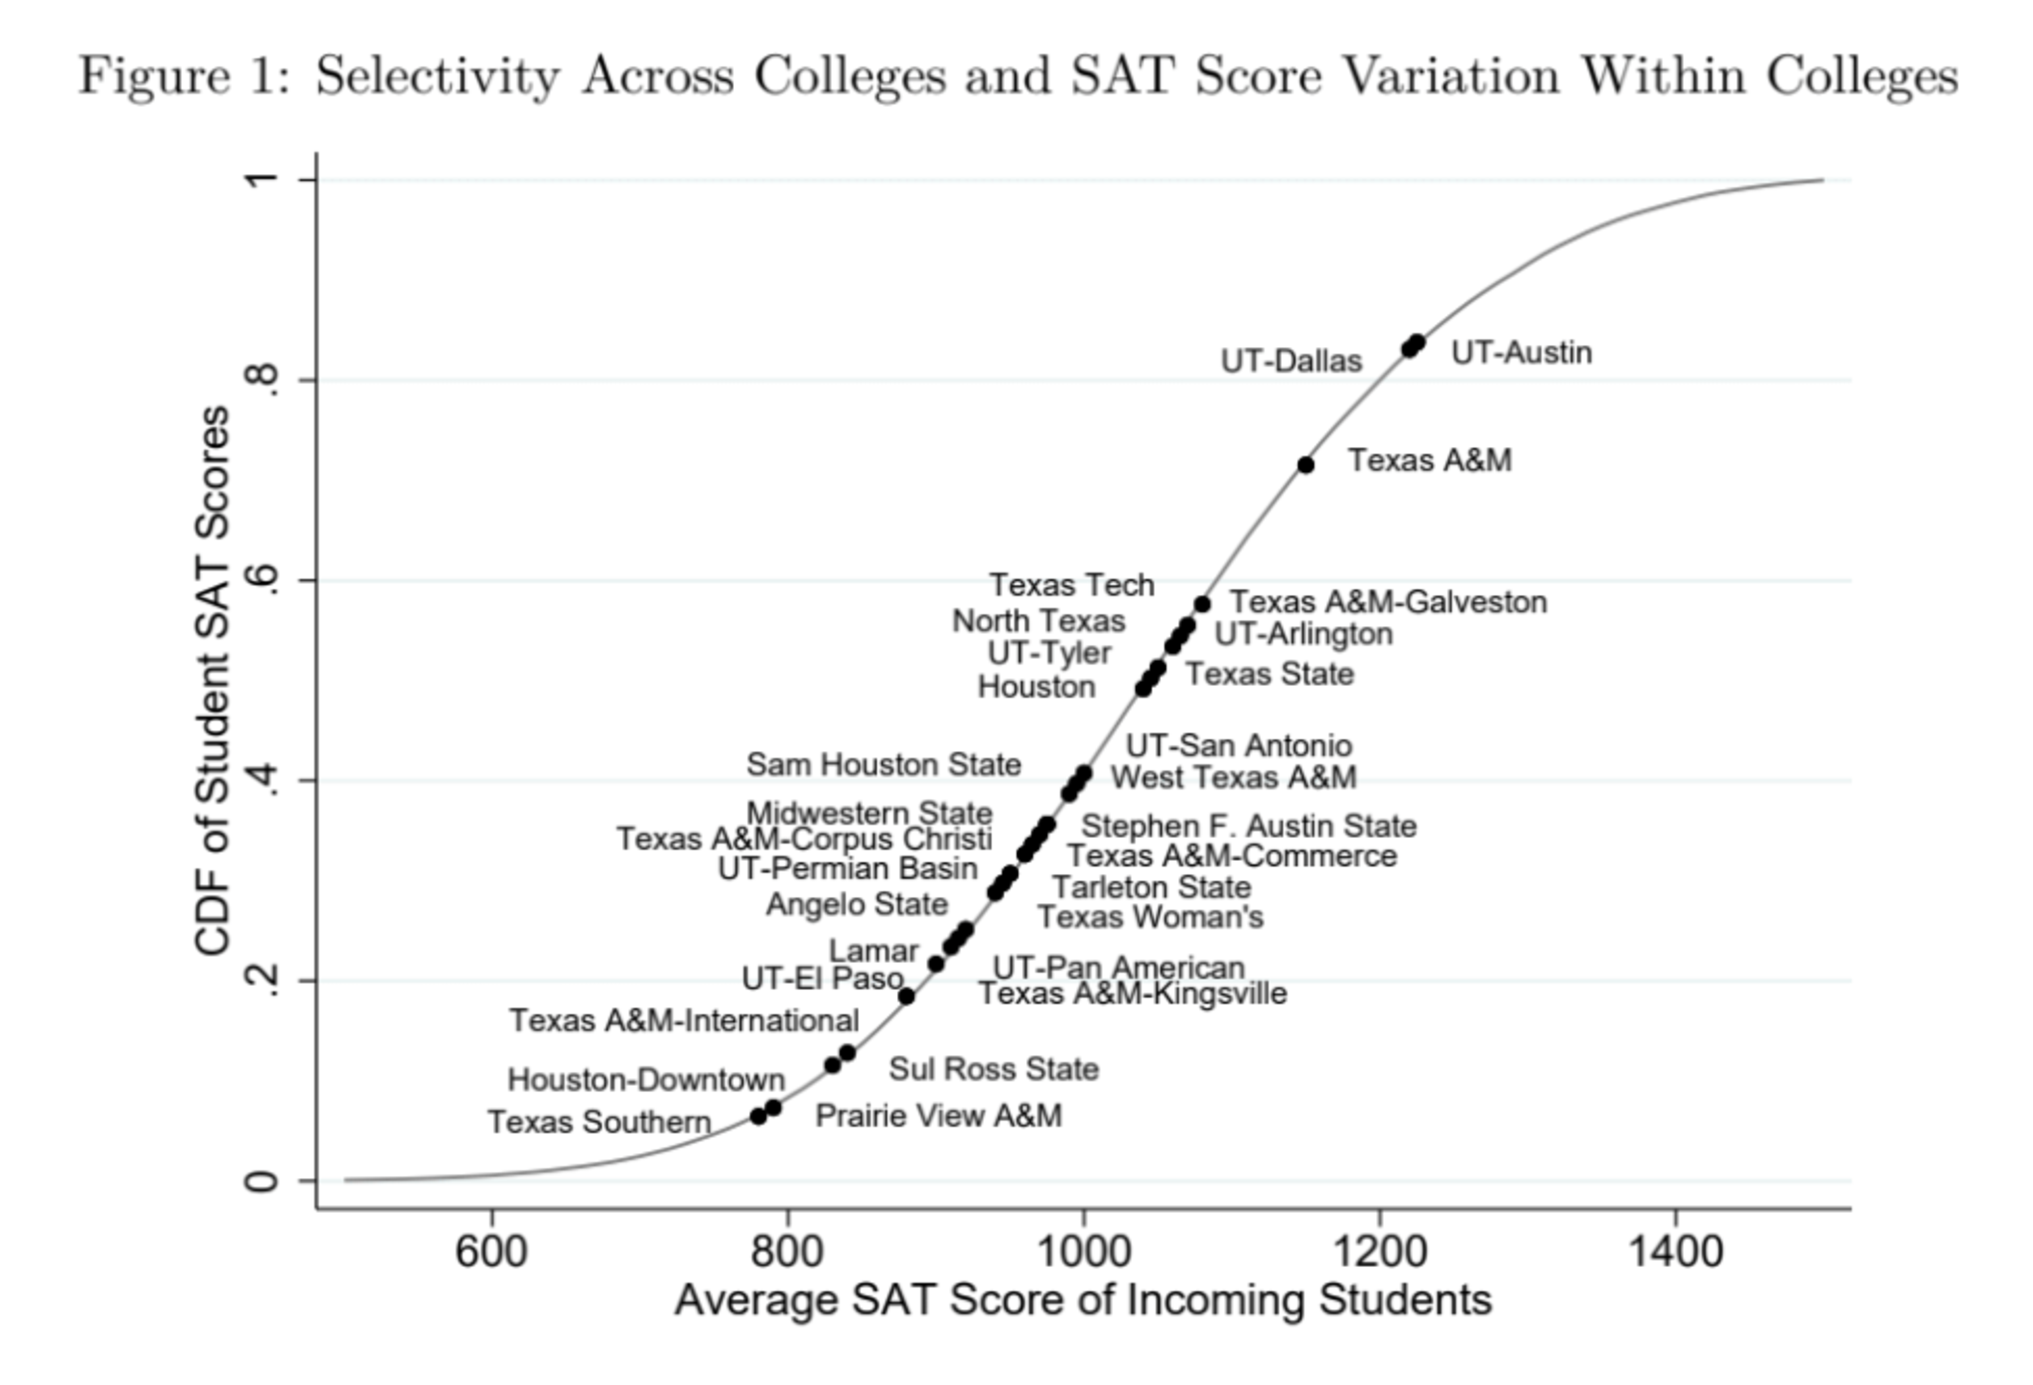
\includegraphics[width = 0.8\linewidth]{mountjoy-colleges}
\end{frame}

\begin{frame}
	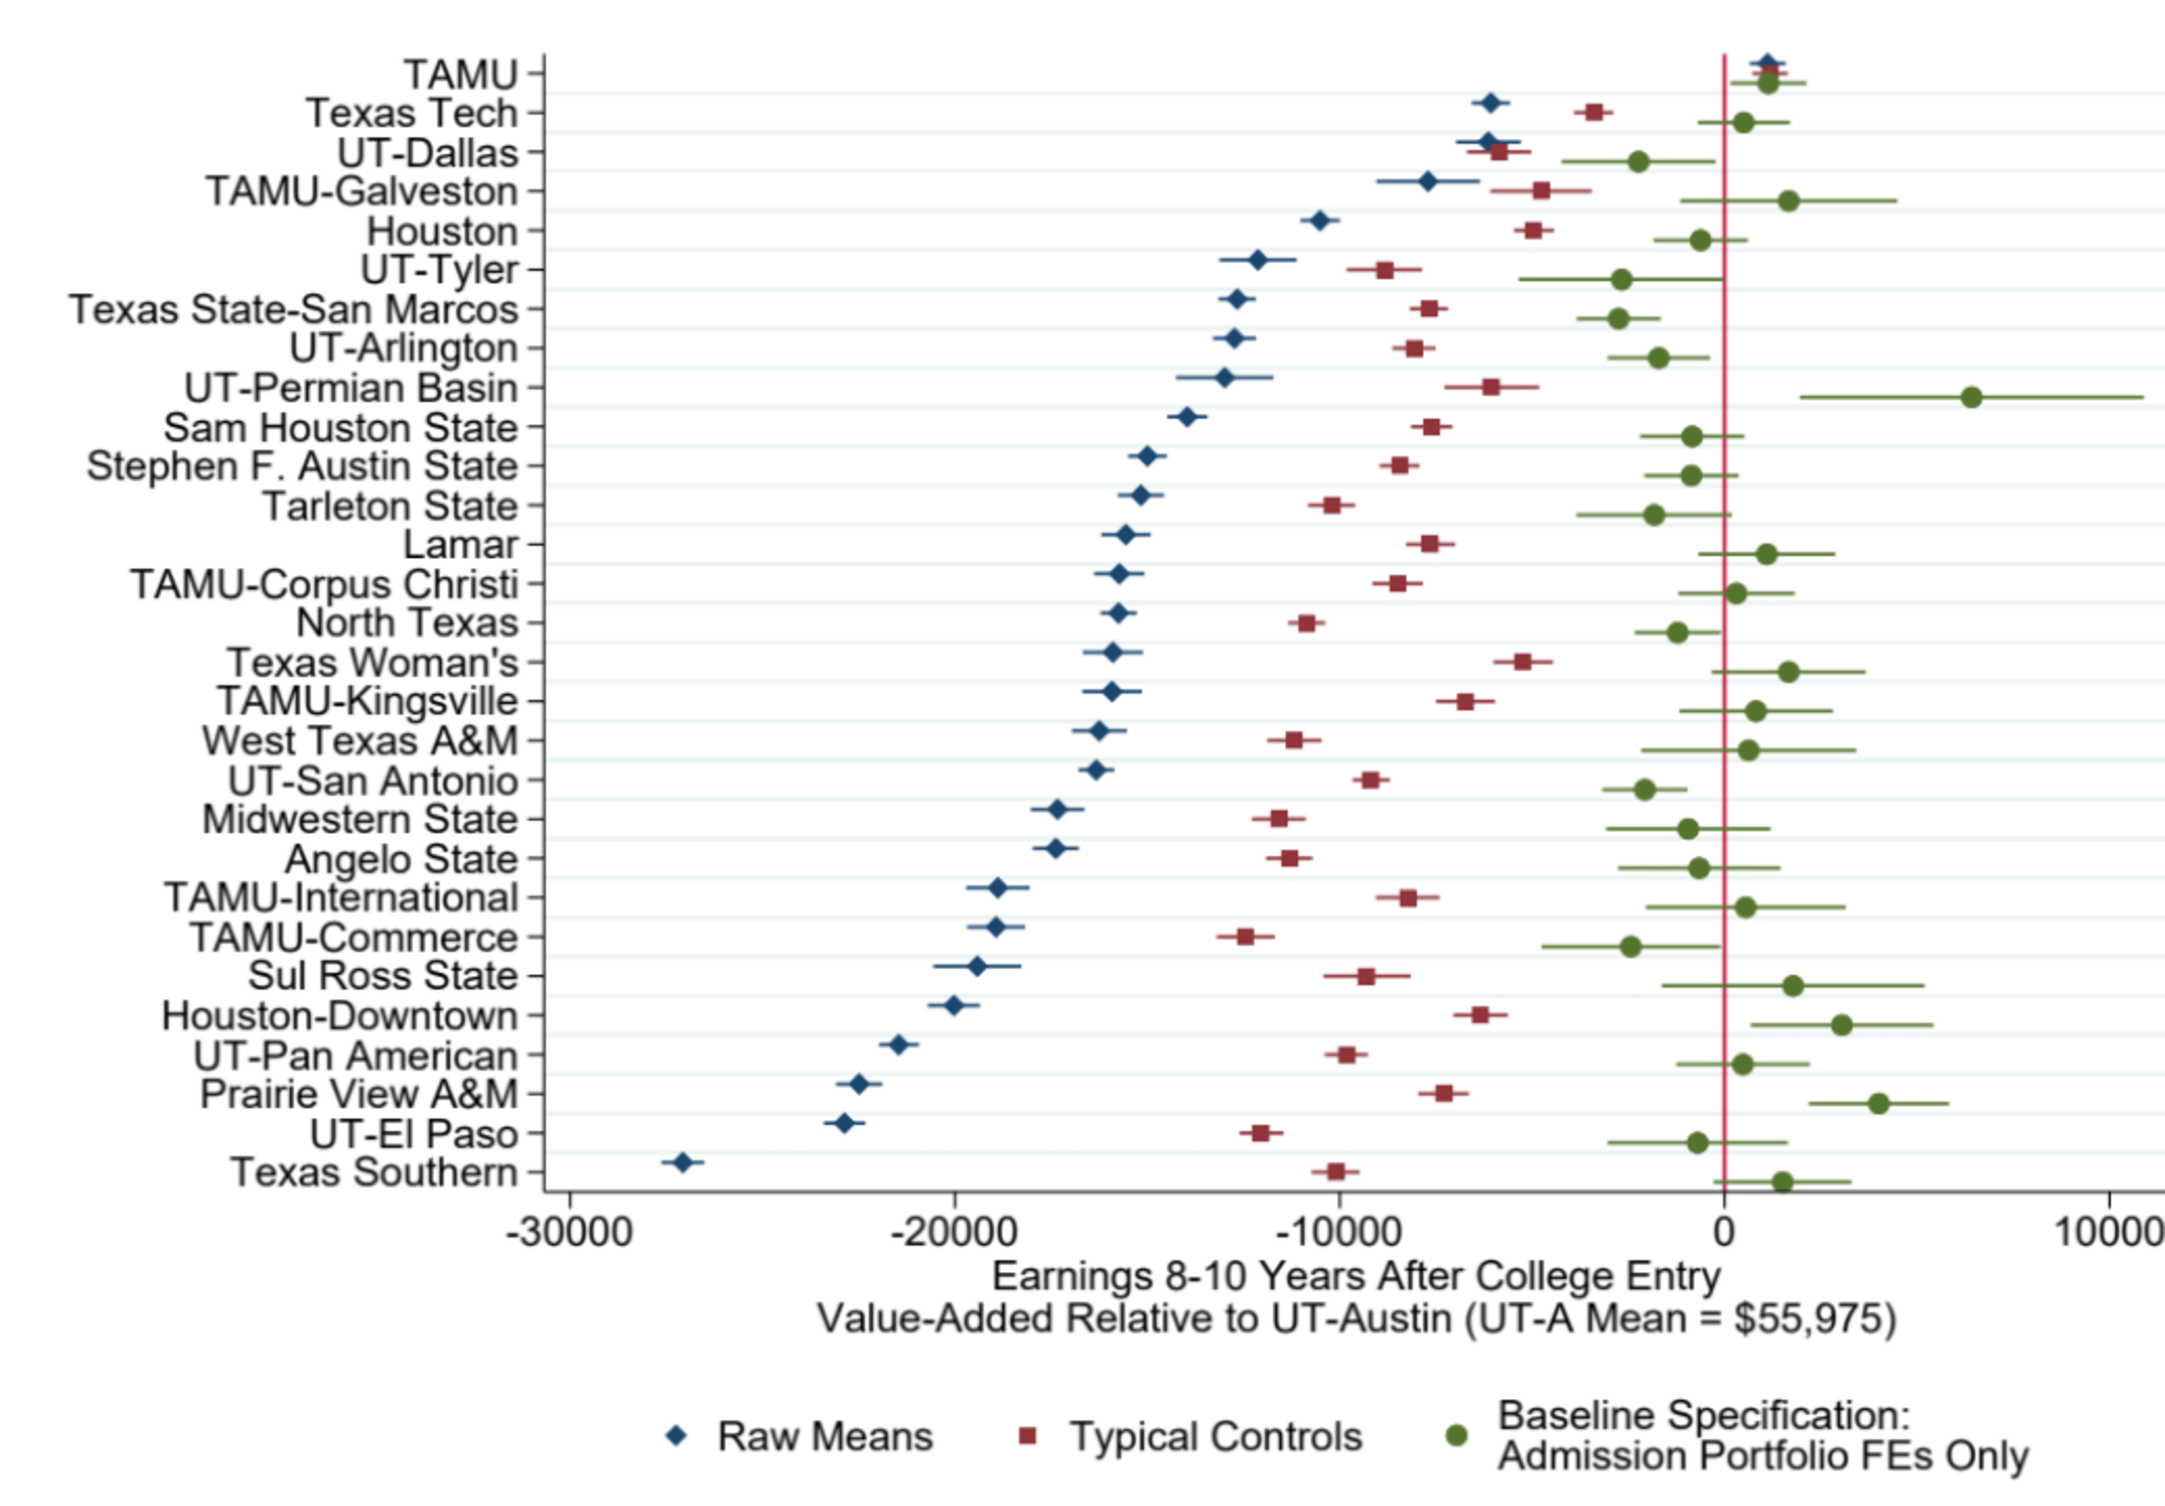
\includegraphics[width = 0.7\linewidth]{mountjoy-earnings}

\begin{itemize}
	\item 
	大学間で所得に有意な差はありますが、それほど大きくはありません。
	
	\item
	プレステージが高いことが必ずしも高い所得を意味するわけではありません（例：テキサス大オースティン校 vs パーミアンベースン校）。
\end{itemize}
\end{frame}


\begin{frame}{付加価値の高い大学は何をしているのか}
	大学卒業率が高い、STEM 分野の卒業率が高い、石油・ガス産業への就職率が高いなど \\
	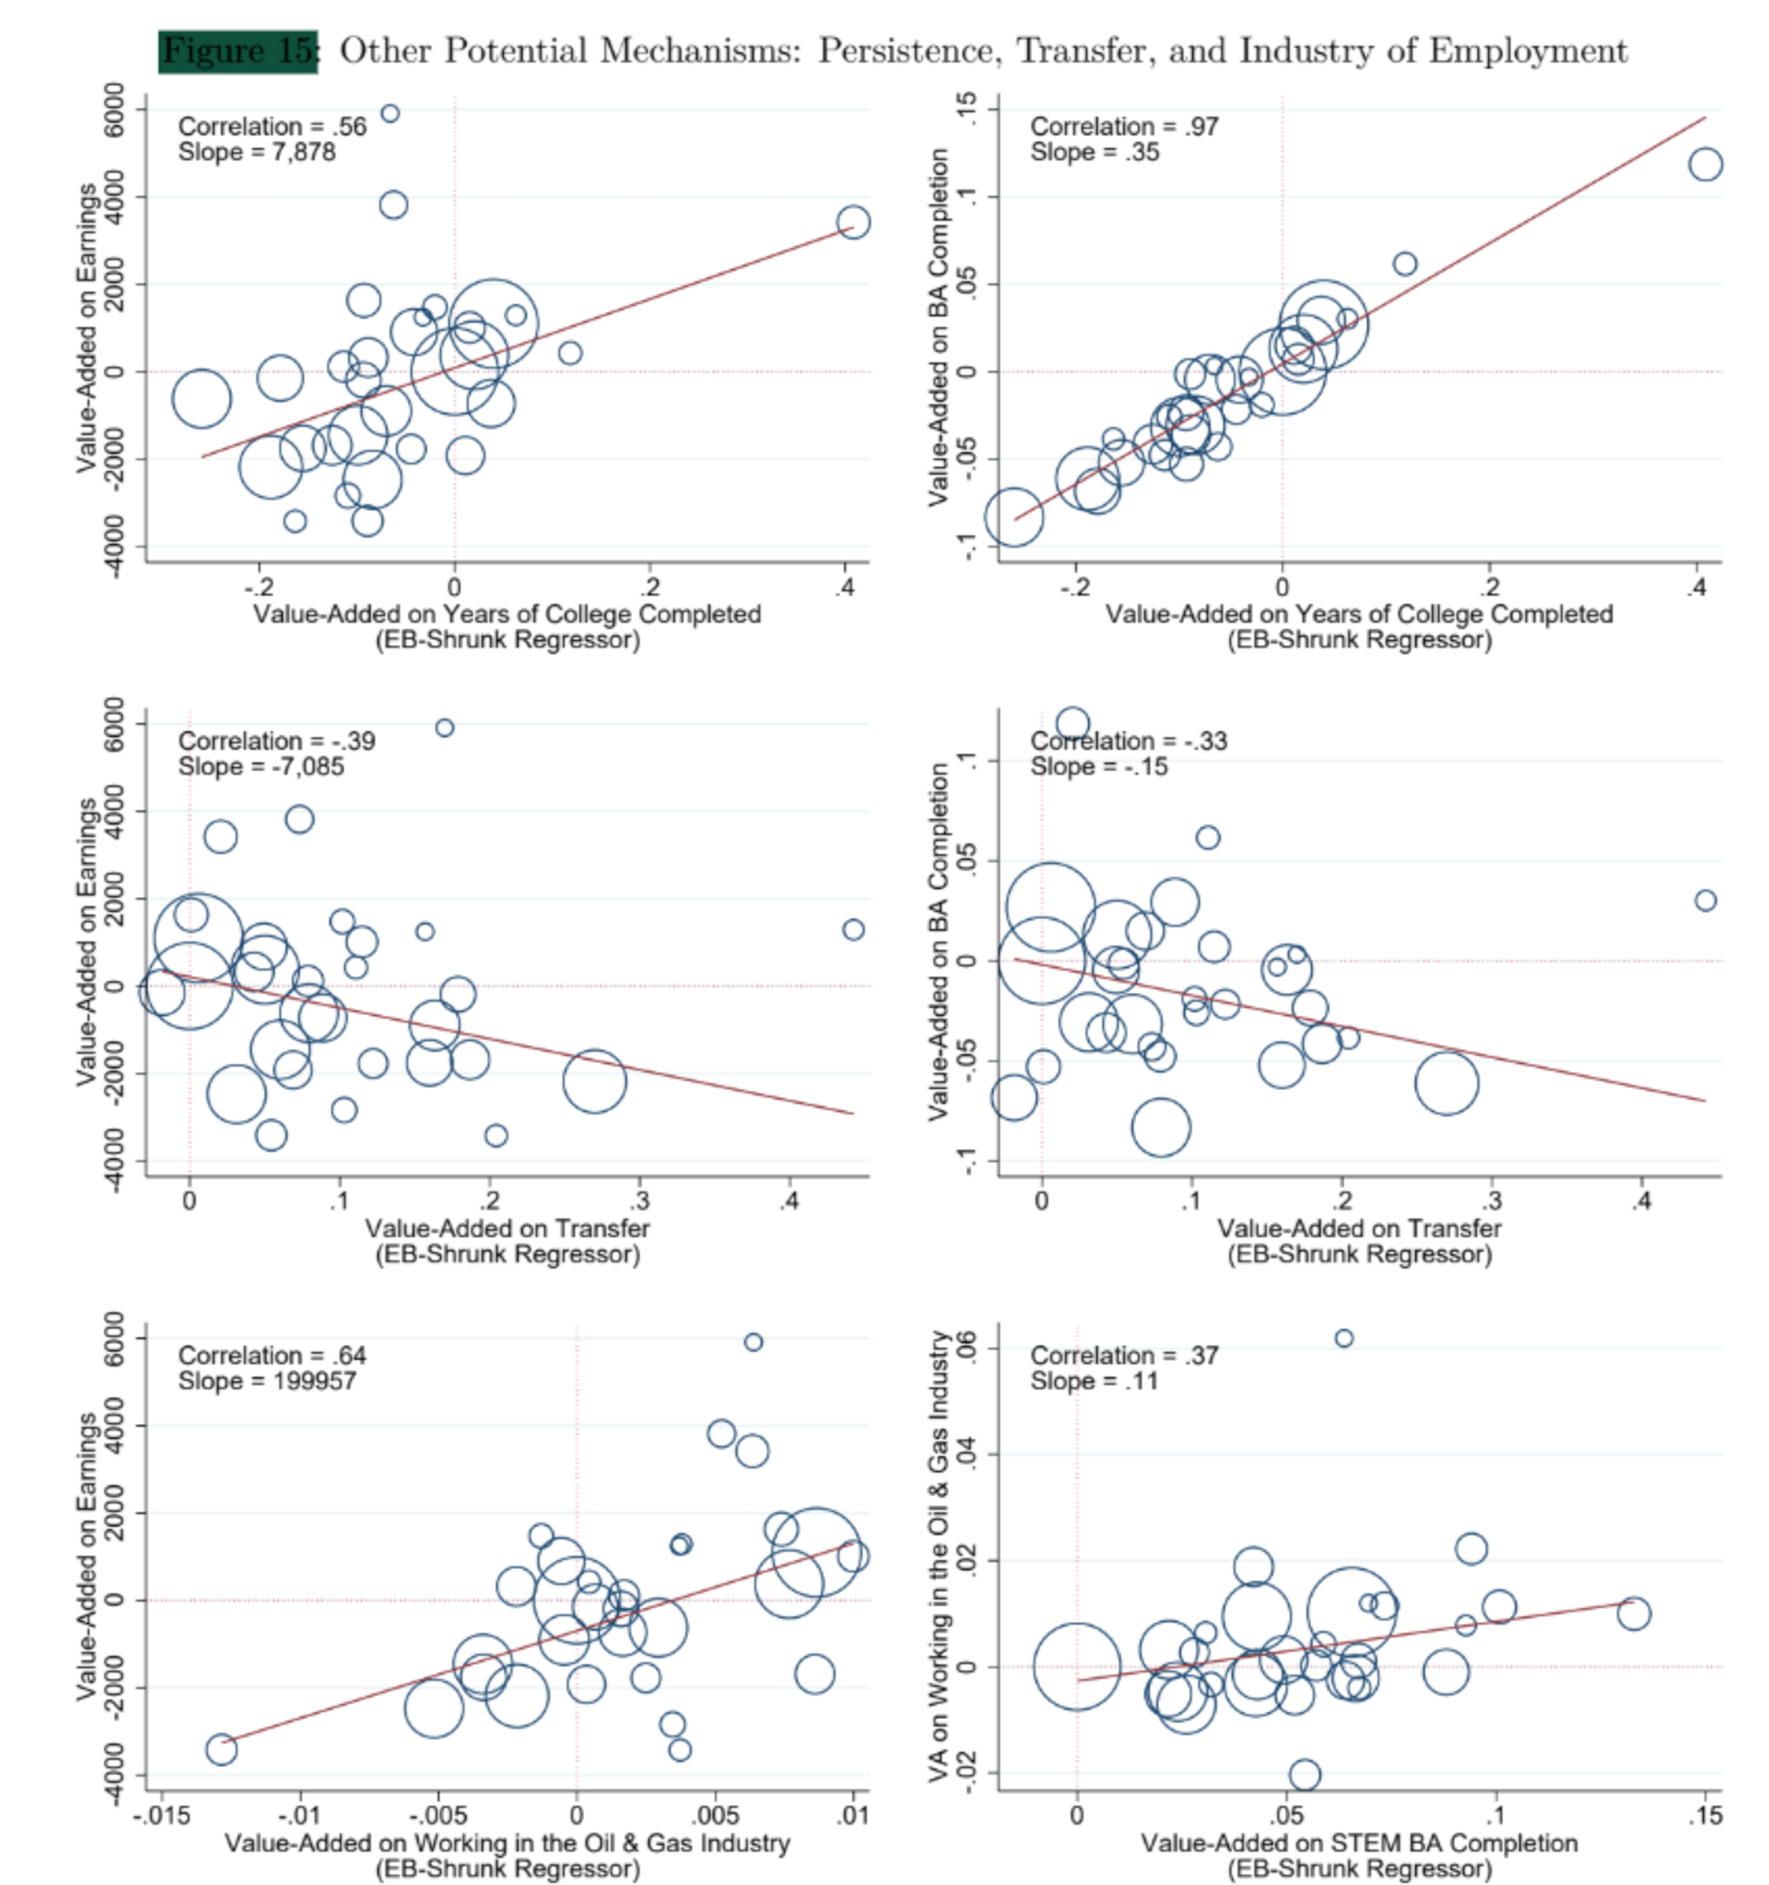
\includegraphics[width = 0.5 \linewidth]{mountjoy-mechs}
\end{frame}


\begin{frame}{Chetty, Deming, Friedman (2025)} 
	
	\begin{wideitemize}
		\item
		いくつかの Ivy+ 校（アイビーリーグ、スタンフォード、MIT、シカゴ、デューク）の合格データと納税所得データを組み合わせて分析しました。
		
		\item
		補欠合格（ウェイトリスト）から合格した学生と、合格しなかった学生を比較しました。
		\begin{itemize}
			\item 
			ある Ivy+ 校での補欠合格は、他の Ivy+ 校での結果を予測しません。
		\end{itemize}	
		\item
		Dale and Krueger と同様に、彼らは\emph{平均}所得に対する大きな影響は見出しませんでした。
		
		\item
		しかし、「エリート」なアウトカムに対しては影響がありました。所得上位 1% に入る確率、「エリート企業」での勤務、 「エリート」大学院への進学などです。
	\end{wideitemize}
	
\end{frame}

\begin{frame}
	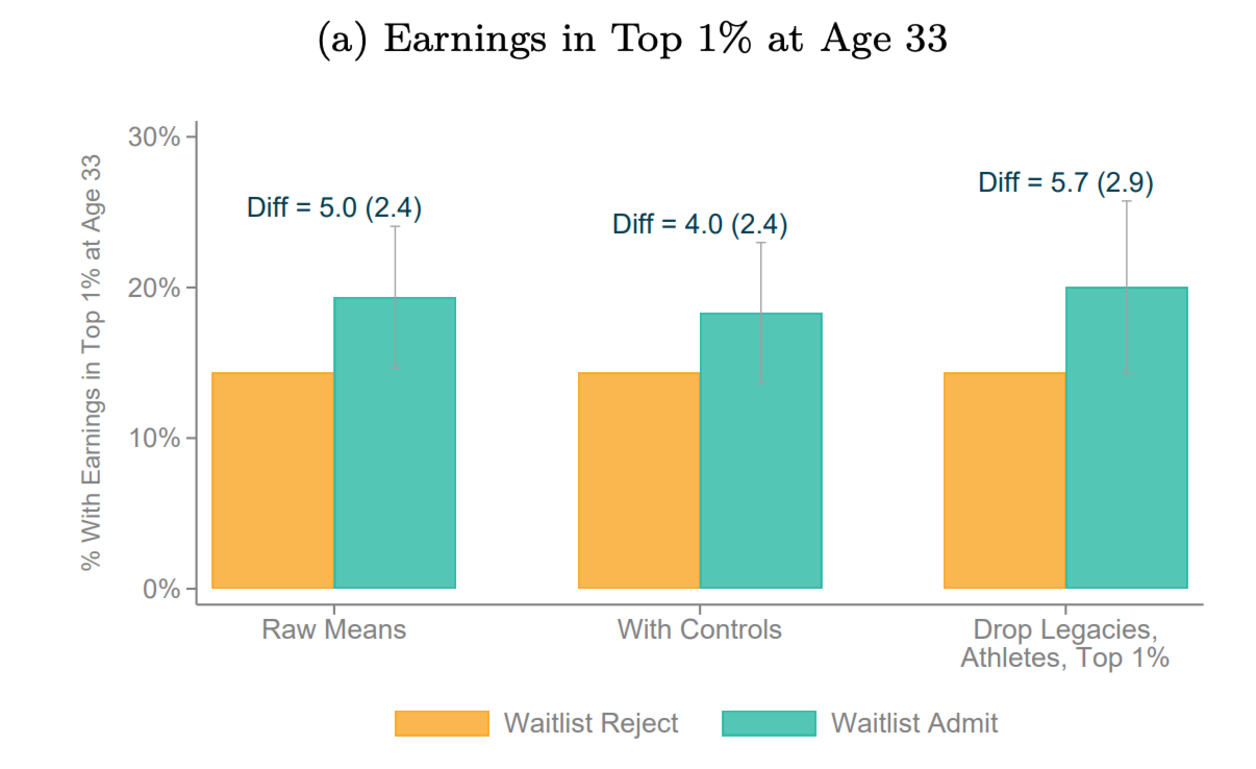
\includegraphics[width = 0.8\linewidth]{chetty-top1}
\end{frame}

\begin{frame}
	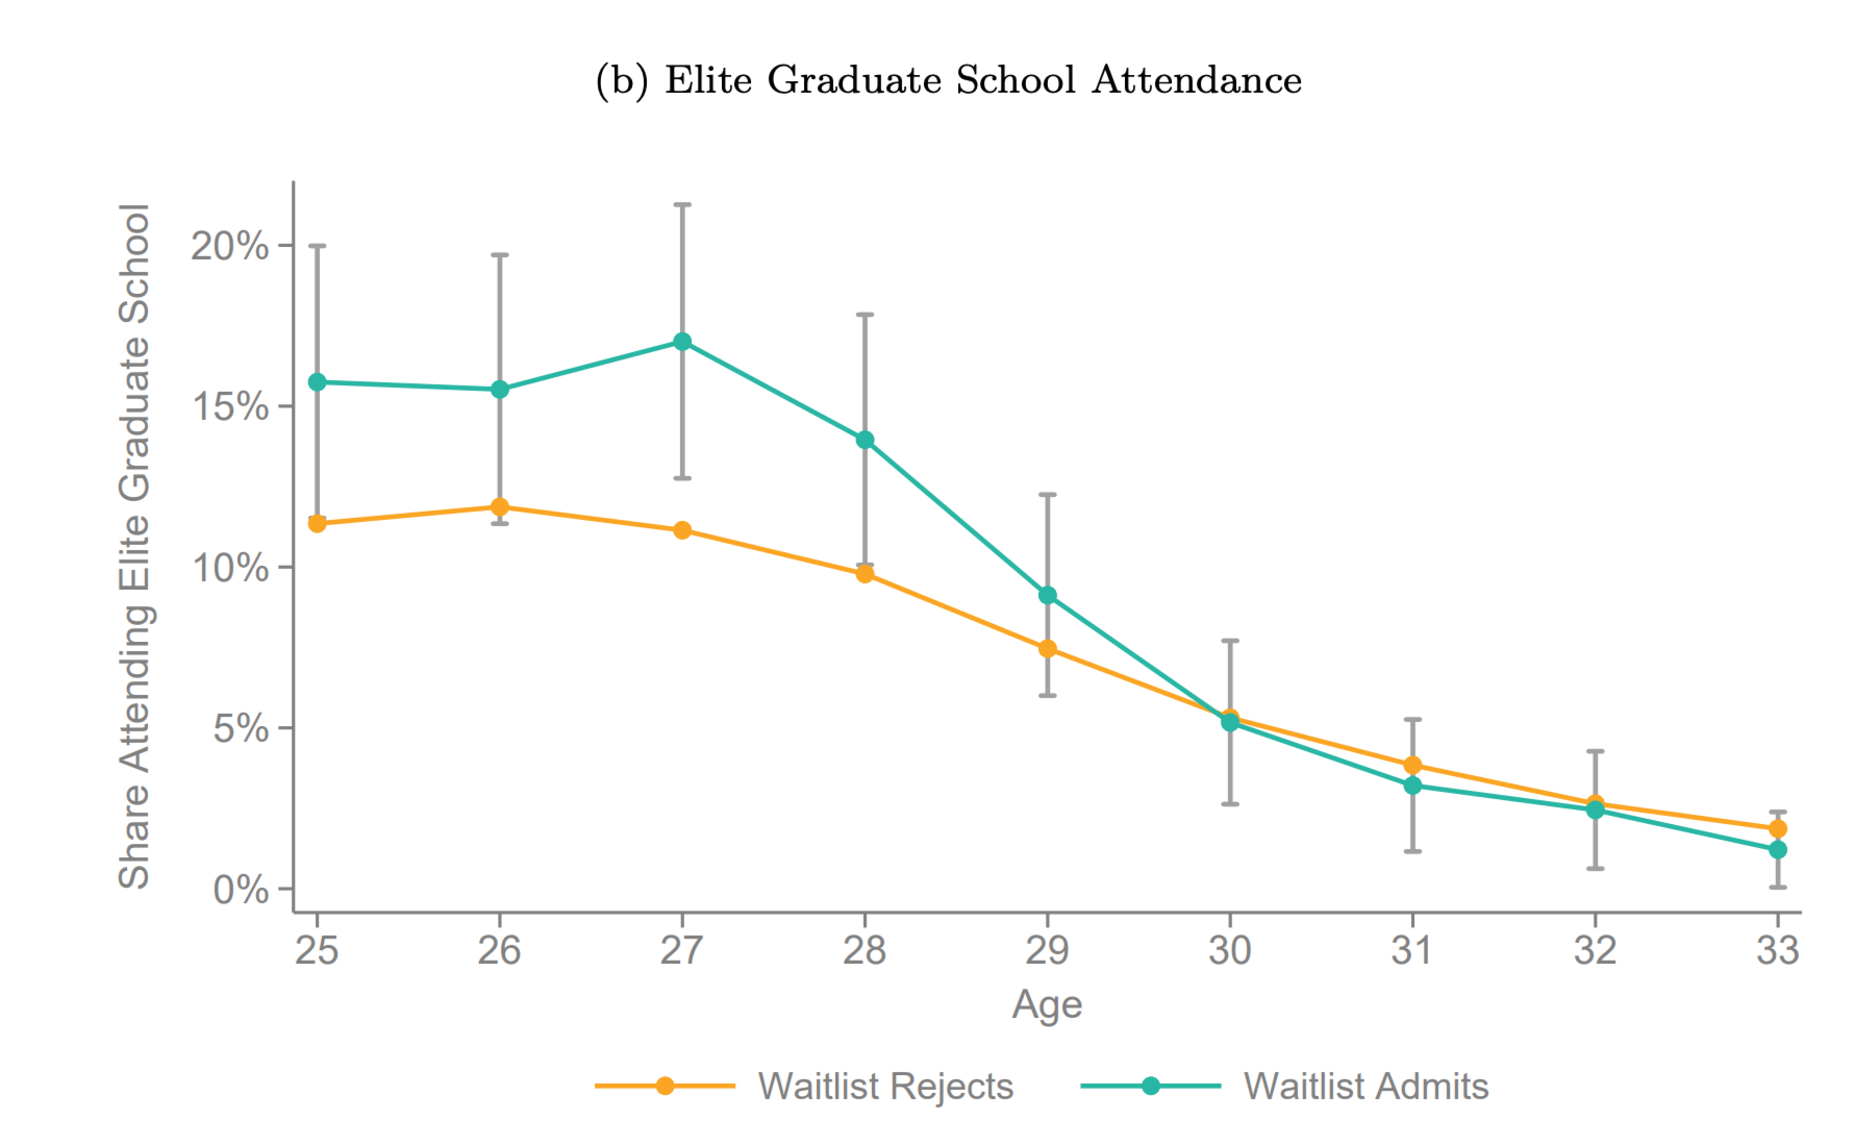
\includegraphics[width = 0.8\linewidth]{chetty-gradschool}
\end{frame}

	\begin{frame}{アウトライン}

	\textcolor{red!75!green!50!blue!25!gray}{1. 多変量回帰と OLS の導出}$\checkmark$
	\vspace{0.8cm}
	
	\textcolor{red!75!green!50!blue!25!gray}{2. 回帰と因果関係}$\checkmark$
	\vspace{0.8cm}
	
	3. 回帰に関するその他のトピック
	
	\end{frame}

\begin{frame}{その他のトピック 1：多重検定（多重比較）}
	\begin{wideitemize}
		\item
		グループ間での因果的効果の違いをテストする方法を見てきました。
		
		\pause
		\item
		ここでは「貧しい学生 vs 裕福な学生」という1つの次元の異質性を考えました。しかし、他のグループについての異質性にも興味があるかもしれません。 \smallskip
			\begin{itemize}
				\item
				男性の方が女性よりも効果が大きいか？ \smallskip
				
				\pause
				\item
				アスリートの方が非アスリートよりも効果が大きいか？ \smallskip
				
				\pause
				\item
				裕福な家庭の男性アスリートの方が、貧しい家庭の女性非アスリートよりも効果が大きいか？
		   \end{itemize}
	   
	  \pause
	  \item
	  テストしたい仮説の数は非常に多くなる可能性があります！
	  
	  \pause
	  \item
	  これは「\textbf{多重検定}（multiple hypothesis testing）」問題と呼ばれる状況を引き起こします。
	\end{wideitemize}	
\end{frame}


\begin{frame}{多重検定（続き）}
	\begin{wideitemize}
		\item
		思い出してください： $p$ 値は、（漸近的に）処置効果がないという帰無仮説の下で、 $p < 0.05$ となる確率が 5% になるように構築されています。
		
		\pause
		\item
		したがって、全人口に対して有意な効果があるかテストする場合、真に効果がなければ、棄却される確率は 5% だけです。
		
		\pause
		\item
		しかし、まず男性について有意な効果をテストし、
		次に女性についてもテストしたとしましょう。
		
		\pause
		\item
		どちらのグループにも有意な効果が全くない場合、少なくとも1つの有意な結果が見つかる確率はどの程度でしょうか？

	\end{wideitemize}
\end{frame}


\begin{frame}
	\begin{wideitemize}
		\item 
		男性と女性のサンプルが独立に抽出されているとします。
		
		\item
		有意な結果の数を $N_{sig}$ とします。
		\begin{align*}
		&P( N_{sig} \geq 1  ) = \pause{} 1 - P(N_{sig} =0)  \pause{} \\
		&= 1 - P(\text{女性が有意でない かつ 男性が有意でない}) \pause{} \\
		& = 1 -P(\text{女性が有意でない}) P(\text{男性が有意でない}) \pause{} \\ 
		& = 1-.95^2 \pause{} =  0.0975
		\end{align*}
	
	\item
	したがって、どちらのグループにも真の効果がない場合でも、約 10% の確率で少なくとも1つの有意な効果が見つかってしまいます。
	
	\pause
	\item
	同じ論理で、 $K$ 個の独立なグループについて帰無仮説をテストし、真の効果がすべて 0 である場合、帰無仮説を棄却してしまう確率は \pause $1 - 0.95^K$ となります。
\end{wideitemize}
\end{frame}


\begin{frame}
$K$ 個の独立なグループ（処置効果は 0）において、少なくとも1つのサブグループで有意な効果が見つかる確率： \\
		\begin{tabular}{rr}
		$K$& $1-0.95^K$ \\ \hline 
		1 & 0.05 \\
		2 & 0.0975 \\ \pause{}
		3 & \pause{} 0.1426 \\
		5 &\pause{} 0.2262 \\
		10 & \pause{} 0.4013\\
		100 & \pause{} 0.9941
	\end{tabular}

\end{frame}


\begin{frame}{多重検定のシミュレーション}
\begin{wideitemize}
	\item
	「Current Population Survey」の平均時給の調査データがあります。
	
	\item
	確率 1/2 で 1 となる偽の処置 $D_i$ を生成します。
	
	\pause
	\item
	この処置の真の因果的効果は何でしょうか？ \pause もちろん 0 です。
	
	\pause
	\item
	この偽の処置を 1000 回シミュレーションし、以下を推定します：
	
	\begin{enumerate}
		\item 
		全州をプールした処置効果
		
		\item
		最初の 10 州それぞれの処置効果
		
		\item
		全 50 州それぞれの処置効果
		
	\end{enumerate}

	\pause
	\item
	そして、少なくとも1つの有意な推定値が得られるシミュレーションの割合を計算します。

\end{wideitemize}	
	
\end{frame}


\begin{frame}
	\only<1-2>{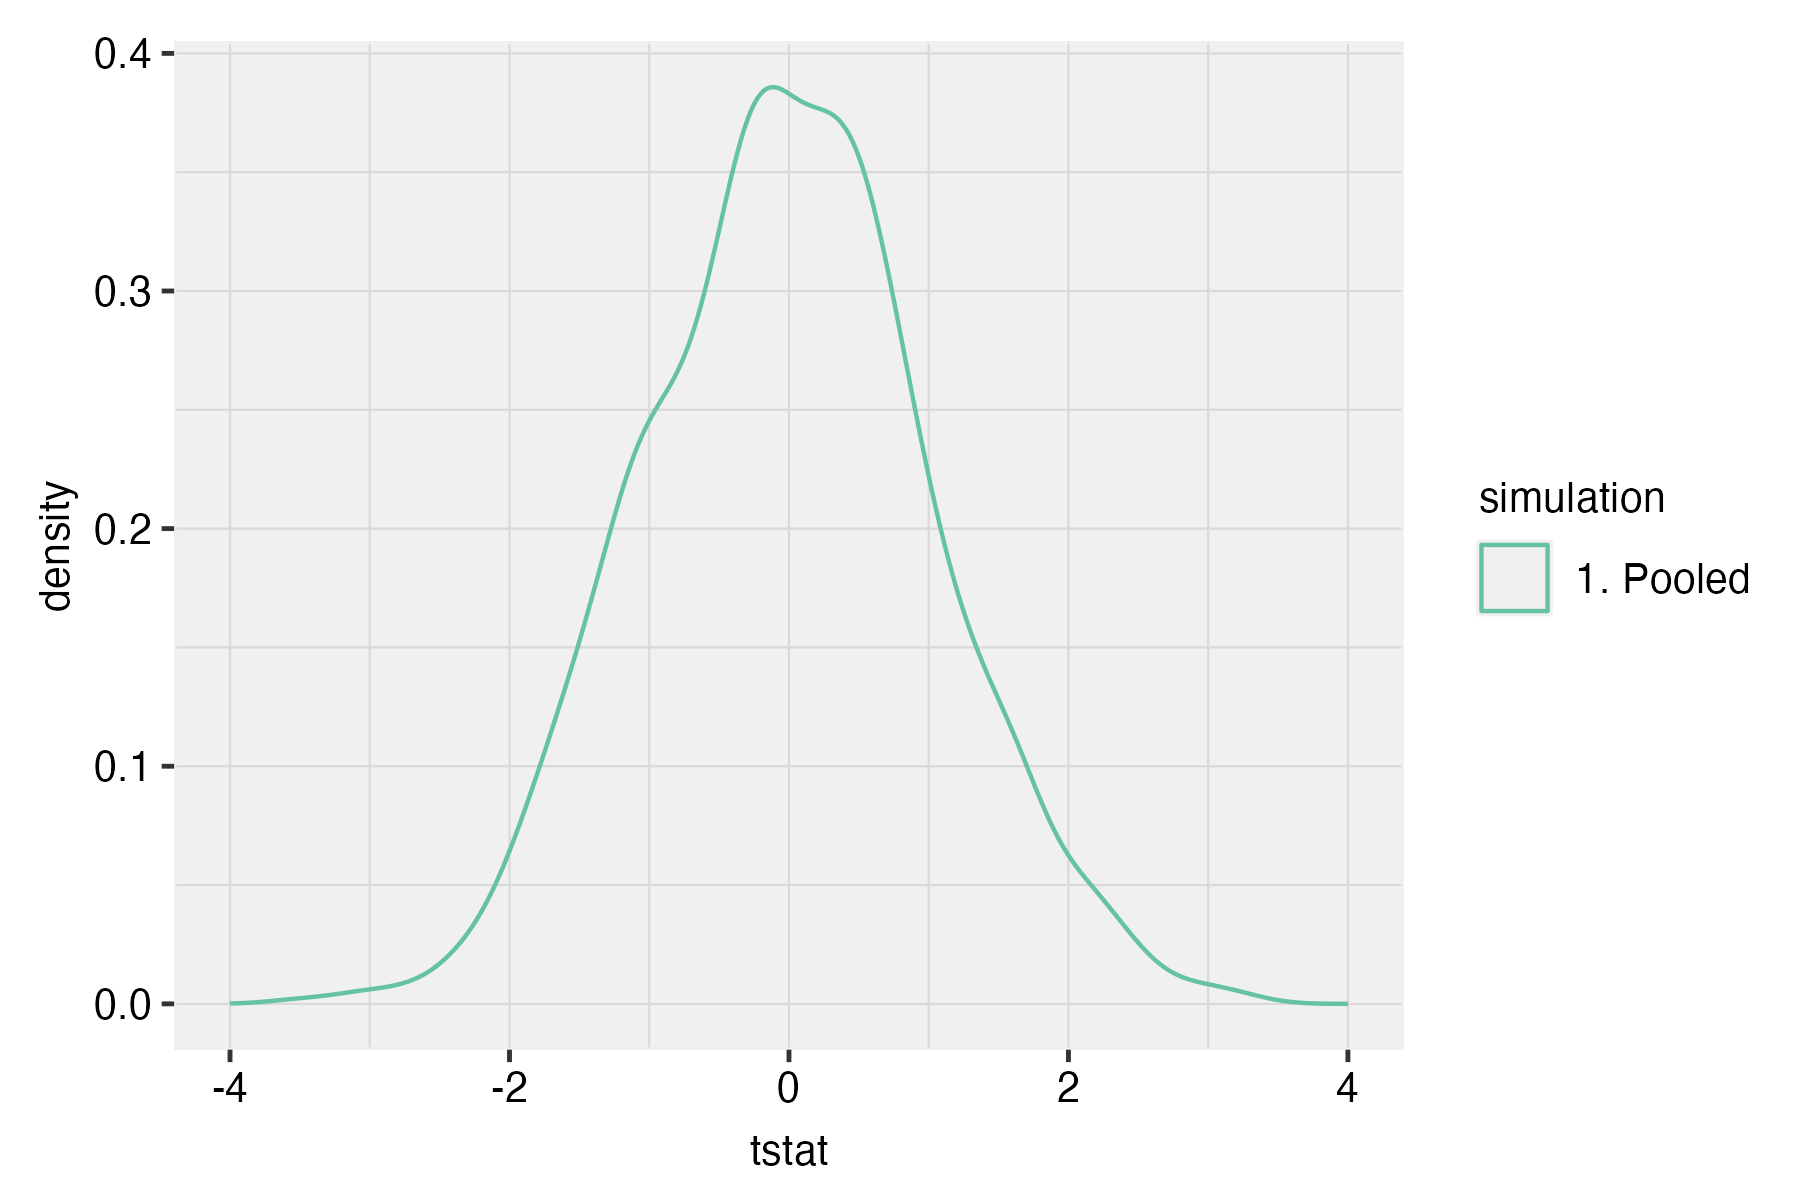
\includegraphics[width = 0.8\linewidth]{multiple-hypothesis-testing-pooled-only}}
	\only<3-4>{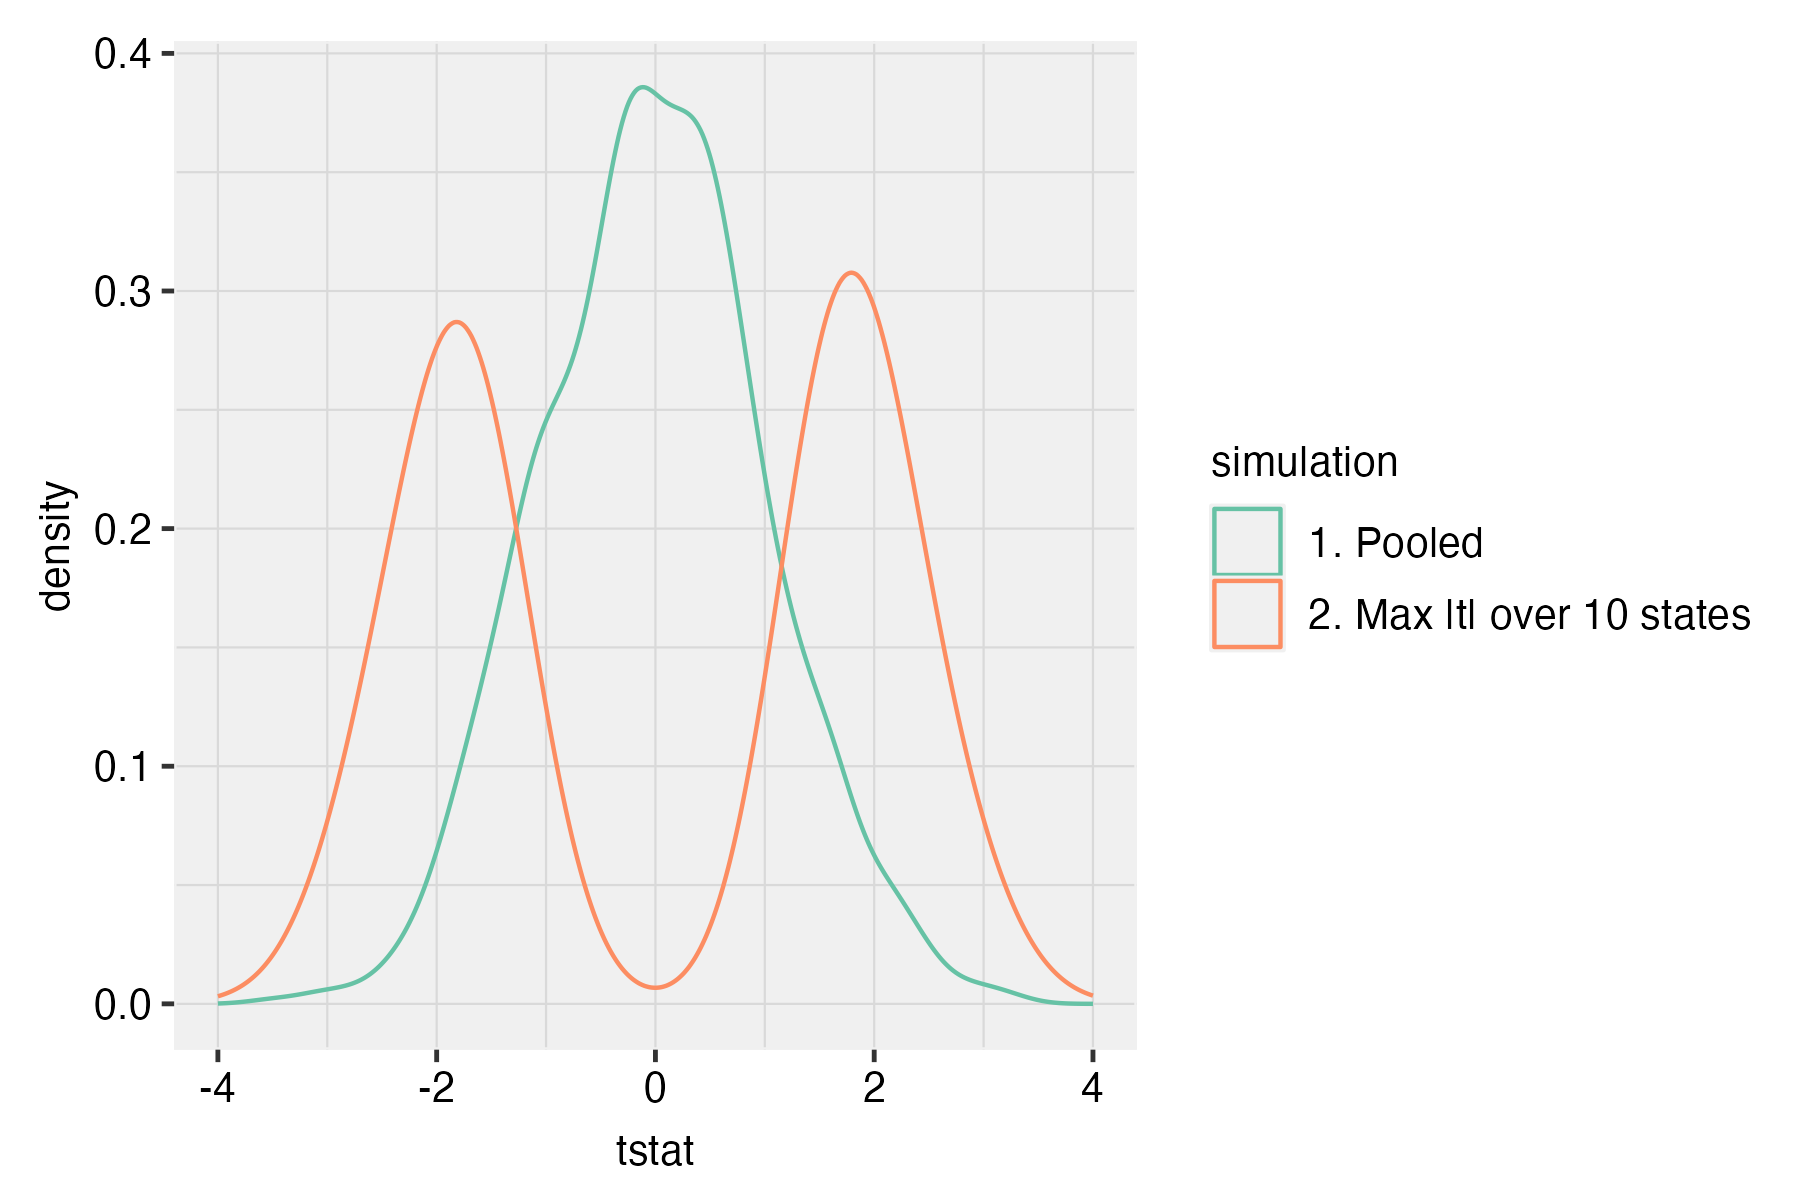
\includegraphics[width = 0.8\linewidth]{multiple-hypothesis-testing-pooled-plus-10}}
	\only<5-6>{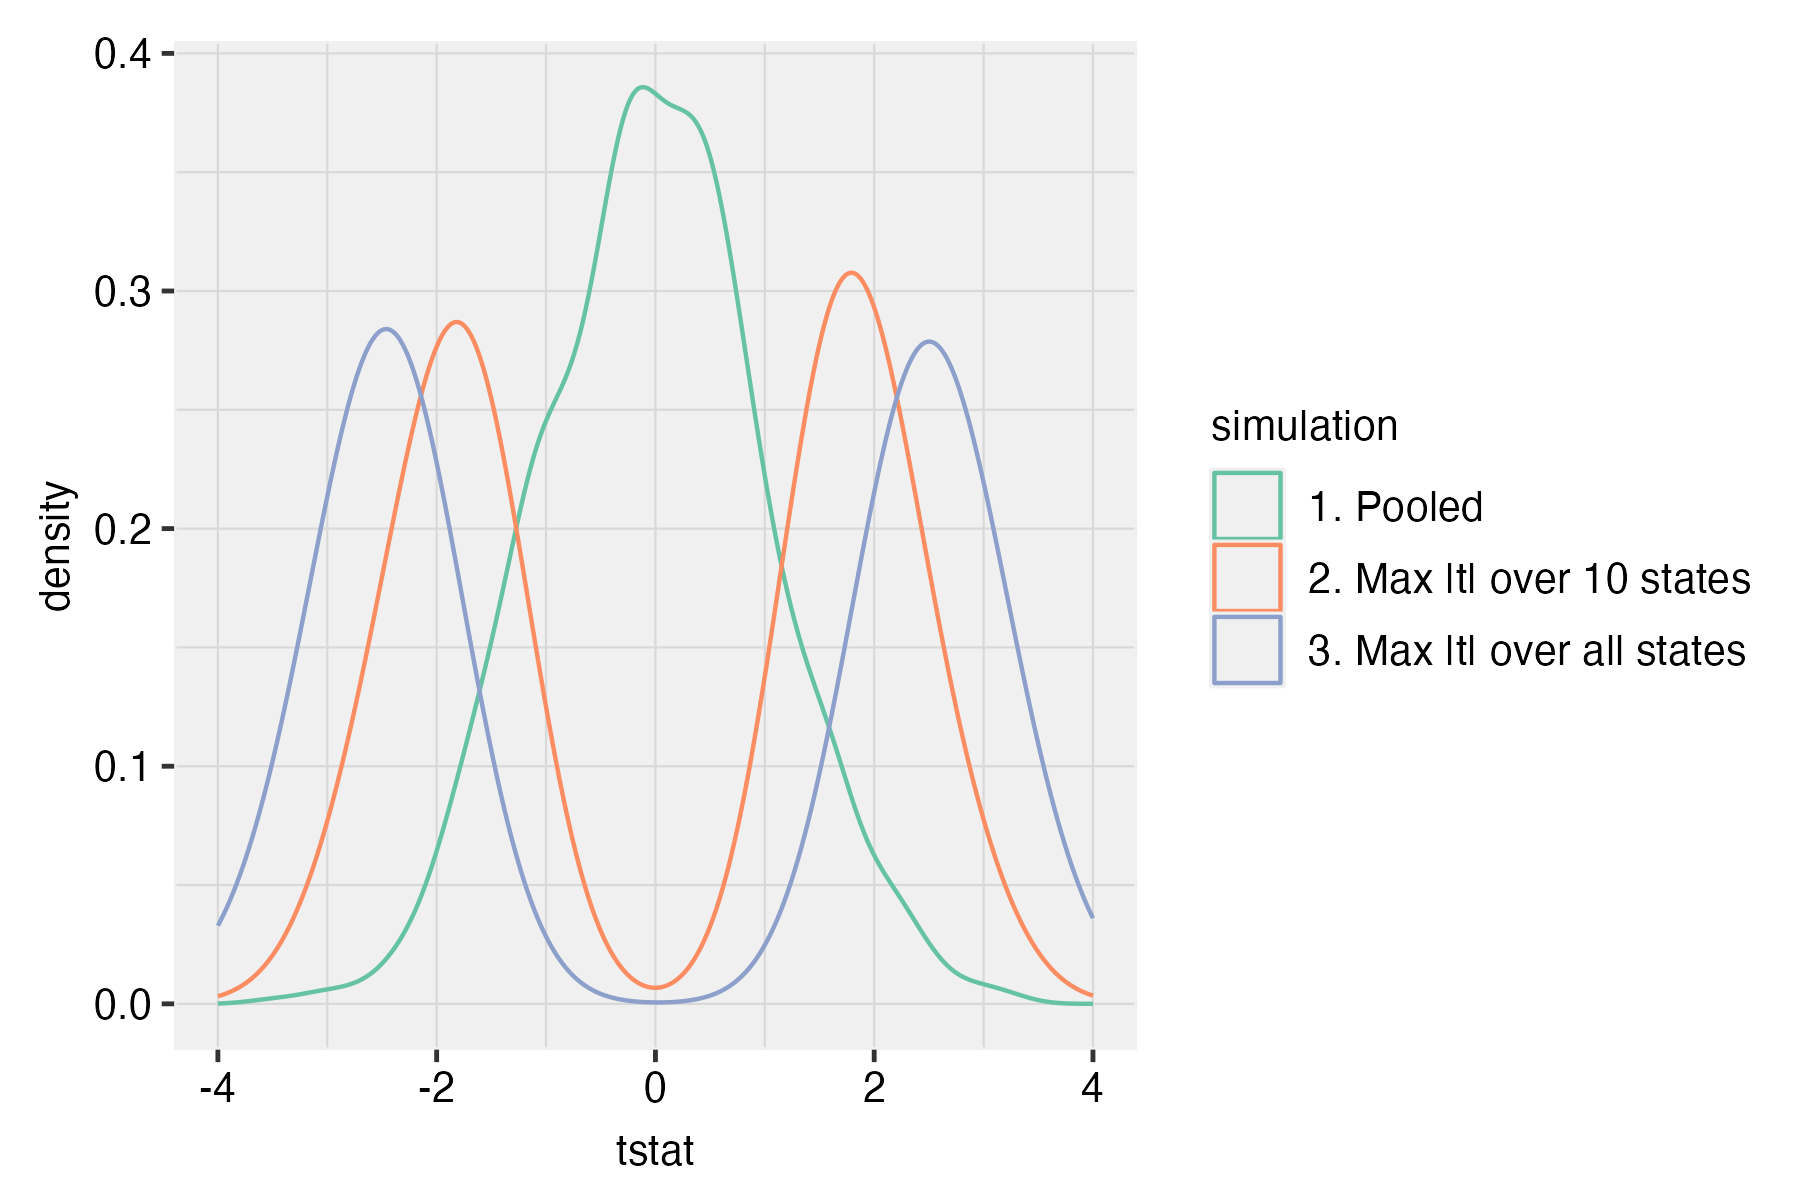
\includegraphics[width = 0.8\linewidth]{multiple-hypothesis-testing-all}}
	
	\only<2>{	
		\begin{wideitemizeshort}
			\item 全州をプールしてテストした場合、6% の確率で有意な効果が見つかります。
		\end{wideitemizeshort}
		}
	
		\only<4>{	
		\begin{wideitemizeshort}
			\item 10州を個別にテストした場合、41% の確率で（どこかの州で）有意な効果が見つかります。
		\end{wideitemizeshort}
	}
	
	
	\only<6>{	
		\begin{wideitemizeshort}
			\item 50州を個別にテストした場合、93% の確率で（どこかの州で）有意な効果が見つかります。
		\end{wideitemizeshort}
	}
	
\end{frame}

\begin{frame}{多重検定の補正}
\begin{wideitemize}
	\item
	多重検定の最も単純な補正方法は、\textbf{ボンフェローニ}（Bonferroni）補正です。
	
	\pause
	\item
	$K$ 個の個別の仮説を 5% 水準でテストする代わりに、それぞれを $5/K$% 水準でテストします。
	
	\pause
	\item
	すると：
	$$P( N_{sig} > 0  ) \leq \sum_k P( \text{k が有意}  ) = K (0.05/K) = 0.05 $$
	
	\pause
	\item
	これは仮説が独立でない場合（例：グループが重複している場合）でも機能します。
	
	\pause
	\item
	欠点：仮説の数が多いと、個々の仮説に対する検出力が非常に低くなります（例：99.9% 信頼区間は非常に広くなります）。 \\ \pause{}
	また、このテストは一般に保守的であり、有意な効果が見つかる確率は 5% 未満になる傾向があります。
		
\end{wideitemize}	
\end{frame}


\begin{frame}
	ボンフェローニ補正なし、および補正ありで、少なくとも1つの仮説を棄却する確率： \\
	\begin{tabular}{lrr}
		シミュレーション & 補正なし & 補正あり \\ \hline
		プール & 0.06 & 0.05 \\
		10 州 & 0.41 &  0.05 \\
		50 州 & 0.93 & 0.04
	\end{tabular}
\end{frame}


\begin{frame}{その他のトピック 2：結合仮説}
	\begin{wideitemize}
		\item
		時として、\textit{いずれか}のサブグループ（例：いずれかの州）で効果があるかどうかだけを知りたい場合があります。
		
		\pause
		\item
		すべてのサブグループで処置効果が 0 である、という\textbf{結合帰無仮説}をテストすることができます。
		
		\pause
		\item
		もしこれを棄却できれば、少なくとも1つのサブグループで処置効果が 0 ではない強い証拠があると結論づけられます。
		
		\pause
		\item
		どのようにこれを行うのでしょうか？
		
	\end{wideitemize}	
\end{frame}


\begin{frame}
	\begin{wideitemize}
		\item
		$\hat{t}_k$ を仮説 $k$ の $t$ 統計量とします。帰無仮説 $k$ の下で、 $\hat{t}_k \to_d \pause N(0,1)$ です。
		
		\item
		各仮説のサンプルが独立である場合、 $K$ 個すべての帰無仮説が満たされていれば、 $(\hat{t}_1, \dots, \hat{t}_K)' \to_d N(0, \mathbf{I})$ となります。
		
		\item
		\emph{$F$ 統計量} $F = \sum_k \hat{t}_k^2$ を考えます。 \pause 連続写像定理より、 $K$ 個すべての帰無仮説が満たされていれば：
		
		$$F \to_d  \sum_k Z_k^2 \text{ （ただし } Z \sim N(0, \mathbf{I}) \text{）}$$
		これは、自由度 $K$ の\emph{カイ二乗}（$\chi^2$）分布と呼ばれます。
		
		\item
		したがって、 $F$ をカイ二乗分布の 95%タイル（ $c$ とします）と比較することで、 $K$ 個すべての帰無仮説が満たされているかテストできます。 $F > c$ であれば、すべての仮説が妥当であるという考えを棄却します。
		
		\item
		このアプローチは \emph{$F$ 検定}と呼ばれます。
				
	\end{wideitemize}
\end{frame}


\begin{frame}
	すべての州で処置効果が 0 であるという結合帰無仮説を棄却する確率： \\ \vspace{1cm}
	\begin{tabular}{lrr}
		シミュレーション & 個別のテスト & 結合テスト \\ \hline
		プール & 0.06 & 0.06 \\
		10 州 & 0.41 &  0.04 \\
		50 州 & 0.93 & 0.05
	\end{tabular}
\end{frame}


\begin{frame}{$F$ 検定はボンフェローニよりも検出力が高い場合がある}
	\begin{wideitemize}
		\item
		偽の処置を受けた場合に賃金に 6 ドル加算されるようにシミュレーション設定を変更します。
		
		\item
		ボンフェローニを用いると、少なくとも1つの州で有意な効果が見つかるのは 39% の確率に過ぎません。一方、結合帰無仮説は 60% の確率で棄却されます。
		
		\pause
		\item
		あるシミュレーションの例です：
		
		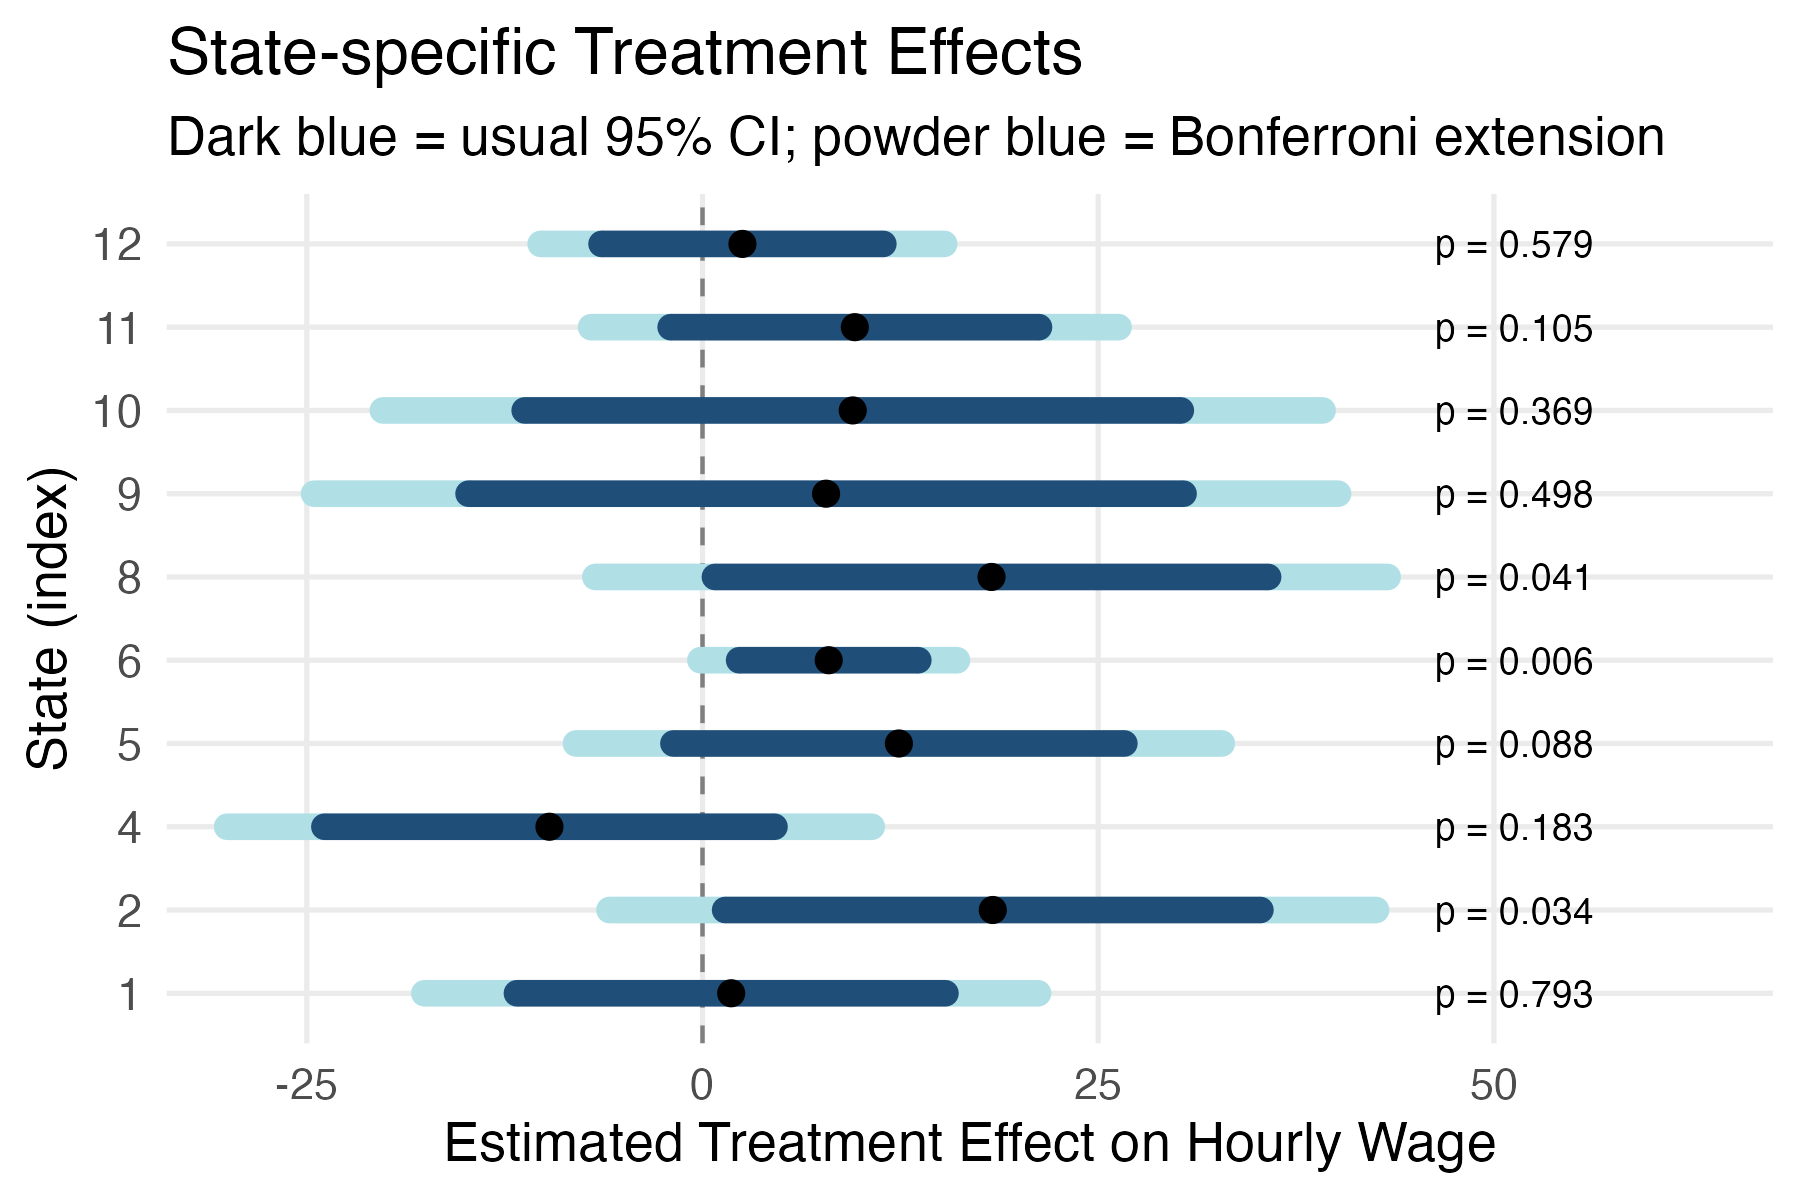
\includegraphics[width = 0.5 \linewidth]{bonf-adj-estimates}\\
		ボンフェローニ補正後、州レベルの効果はどれも有意ではありません。しかし、結合テストの $p$ 値は 0.004 です。
	\end{wideitemize}
\end{frame}


\begin{frame}{複数の回帰係数のテスト}

\begin{wideitemize}
	\item
	複数の回帰係数が 0 であるという帰無仮説をテストしたい場合があります（例：所得と年齢の例で、線形項と2次項の両方が 0 であるか）。
	
	\begin{center}
	\includegraphics[width = 0.3\linewidth]{logwages-quadratic} 
	\end{center}
	
	\item
	この問題に対しても $F$ 検定を使用できます。係数間の相関を考慮に入れる必要があります。
	
	\item
	以前の講義で $\sqrt{N}(\hat\beta - \beta_0) \to_d N(0, \boldsymbol{\Sigma})$ を示しました。帰無仮説 $H_0: \beta = \beta_0$ をテストするには、 $F = \sqrt{N} \hat{\boldsymbol{\Sigma}}^{-\frac{1}{2}} (\hat\beta - \beta_0)$ を使用します。
	
	\item
	これは Stata の \texttt{test} 関数で実装されています。例えば \texttt{test age agesq} は、年齢と年齢の2乗の係数がともに 0 である（＝所得が年齢に依存しない）という帰無仮説をテストします。
\end{wideitemize}	
	

\end{frame}


\begin{frame}
	\includegraphics[width = 0.7\linewidth]{f-test}
\end{frame}


	
\end{document}
